%%% Hlavní soubor. Zde se definují základní parametry a odkazuje se na ostatní části. %%%

%% Verze pro jednostranný tisk:
% Okraje: levý 40mm, pravý 25mm, horní a dolní 25mm
% (ale pozor, LaTeX si sám přidává 1in)
\documentclass[12pt,a4paper,hyphens]{report}
\setlength\textwidth{145mm}
\setlength\textheight{247mm}
\setlength\oddsidemargin{15mm}
\setlength\evensidemargin{15mm}
\setlength\topmargin{0mm}
\setlength\headsep{0mm}
\setlength\headheight{0mm}
% \openright zařídí, aby následující text začínal na pravé straně knihy
\let\openright=\clearpage

%% Pokud tiskneme oboustranně:
% \documentclass[12pt,a4paper,twoside,openright]{report}
% \setlength\textwidth{145mm}
% \setlength\textheight{247mm}
% \setlength\oddsidemargin{14.2mm}
% \setlength\evensidemargin{0mm}
% \setlength\topmargin{0mm}
% \setlength\headsep{0mm}
% \setlength\headheight{0mm}
% \let\openright=\cleardoublepage

%% Vytváříme PDF/A-2u
\usepackage[a-2u]{pdfx}

%% Přepneme na českou sazbu a fonty Latin Modern
\usepackage[czech]{babel}
\usepackage{lmodern}
\usepackage[T1]{fontenc}
\usepackage{textcomp}

%% Použité kódování znaků: obvykle latin2, cp1250 nebo utf8:
\usepackage[utf8]{inputenc}

%%% Další užitečné balíčky (jsou součástí běžných distribucí LaTeXu)
\usepackage{amsmath}        % rozšíření pro sazbu matematiky
\usepackage{amsfonts}       % matematické fonty
\usepackage{amsthm}         % sazba vět, definic apod.
\usepackage{bbding}         % balíček s nejrůznějšími symboly
			    % (čtverečky, hvězdičky, tužtičky, nůžtičky, ...)
\usepackage{bm}             % tučné symboly (příkaz \bm)
\usepackage{graphicx}       % vkládání obrázků
\usepackage{fancyvrb}       % vylepšené prostředí pro strojové písmo
\usepackage{indentfirst}    % zavede odsazení 1. odstavce kapitoly
\usepackage{natbib}         % zajištuje možnost odkazovat na literaturu
			    % stylem AUTOR (ROK), resp. AUTOR [ČÍSLO]
\usepackage[nottoc]{tocbibind} % zajistí přidání seznamu literatury,
                            % obrázků a tabulek do obsahu
\usepackage{icomma}         % inteligetní čárka v matematickém módu
\usepackage{dcolumn}        % lepší zarovnání sloupců v tabulkách
\usepackage{booktabs}       % lepší vodorovné linky v tabulkách
\usepackage{paralist}       % lepší enumerate a itemize
\usepackage{xcolor}         % barevná sazba
\usepackage{hyperref}


%%% Údaje o práci

% Název práce v jazyce práce (přesně podle zadání)
\def\NazevPrace{Implementace platformy pro poskytování BI nástroje Metabase formou SaaS}

% Název práce v angličtině
\def\NazevPraceEN{An Implementation of a Platform for Providing a BI Tool Metabase as a SaaS}

% Jméno autora
\def\AutorPrace{Michael Ševčík}

% Rok odevzdání
\def\RokOdevzdani{2024}

% Název katedry nebo ústavu, kde byla práce oficiálně zadána
% (dle Organizační struktury MFF UK, případně plný název pracoviště mimo MFF)
\def\Katedra{Katedra softwarového inženýrství}
\def\KatedraEN{Department of Software Engineering}

% Jedná se o katedru (department) nebo o ústav (institute)?
\def\TypPracoviste{Katedra}
\def\TypPracovisteEN{Department}

% Vedoucí práce: Jméno a příjmení s~tituly
\def\Vedouci{RNDr. Martin Svoboda, Ph.D.}

% Pracoviště vedoucího (opět dle Organizační struktury MFF)
\def\KatedraVedouciho{Katedra softwarového inženýrství}
\def\KatedraVedoucihoEN{Department of Software Engineering}

% Studijní program a obor
\def\StudijniProgram{Informatika}
\def\StudijniObor{Programování a vývoj software}

% Nepovinné poděkování (vedoucímu práce, konzultantovi, tomu, kdo
% zapůjčil software, literaturu apod.)
\def\Podekovani{%
Poděkování.
}

% Abstrakt (doporučený rozsah cca 80-200 slov; nejedná se o zadání práce)
\def\Abstrakt{%
Abstrakt.
}
\def\AbstraktEN{%
Abstract.
}

% 3 až 5 klíčových slov (doporučeno), každé uzavřeno ve složených závorkách
\def\KlicovaSlova{%
{SaaS} {Business intelligence} {Generický datový model} {Metabase}
}
\def\KlicovaSlovaEN{%
{SaaS} {Business Intelligence} {Generic Data Model} {Metabase}
}

%% Balíček hyperref, kterým jdou vyrábět klikací odkazy v PDF,
%% ale hlavně ho používáme k uložení metadat do PDF (včetně obsahu).
%% Většinu nastavítek přednastaví balíček pdfx.
\hypersetup{unicode}
\hypersetup{breaklinks=true}

%% Definice různých užitečných maker (viz popis uvnitř souboru)
%%% Tento soubor obsahuje definice různých užitečných maker a prostředí %%%
%%% Další makra připisujte sem, ať nepřekáží v ostatních souborech.     %%%

%%% Drobné úpravy stylu

% Tato makra přesvědčují mírně ošklivým trikem LaTeX, aby hlavičky kapitol
% sázel příčetněji a nevynechával nad nimi spoustu místa. Směle ignorujte.
\makeatletter
\def\@makechapterhead#1{
  {\parindent \z@ \raggedright \normalfont
   \Huge\bfseries \thechapter. #1
   \par\nobreak
   \vskip 20\p@
}}
\def\@makeschapterhead#1{
  {\parindent \z@ \raggedright \normalfont
   \Huge\bfseries #1
   \par\nobreak
   \vskip 20\p@
}}
\makeatother

% Toto makro definuje kapitolu, která není očíslovaná, ale je uvedena v obsahu.
\def\chapwithtoc#1{
\chapter*{#1}
\addcontentsline{toc}{chapter}{#1}
}

% Trochu volnější nastavení dělení slov, než je default.
\lefthyphenmin=2
\righthyphenmin=2

% Zapne černé "slimáky" na koncích řádků, které přetekly, abychom si
% jich lépe všimli.
\overfullrule=1mm

%%% Makra pro definice, věty, tvrzení, příklady, ... (vyžaduje baliček amsthm)

\theoremstyle{plain}
\newtheorem{veta}{Věta}
\newtheorem{lemma}[veta]{Lemma}
\newtheorem{tvrz}[veta]{Tvrzení}

\theoremstyle{plain}
\newtheorem{definice}{Definice}

\theoremstyle{remark}
\newtheorem*{dusl}{Důsledek}
\newtheorem*{pozn}{Poznámka}
\newtheorem*{prikl}{Příklad}

%%% Prostředí pro důkazy

\newenvironment{dukaz}{
  \par\medskip\noindent
  \textit{Důkaz}.
}{
\newline
\rightline{$\qedsymbol$}
}

%%% Prostředí pro sazbu kódu, případně vstupu/výstupu počítačových
%%% programů. (Vyžaduje balíček fancyvrb -- fancy verbatim.)

\DefineVerbatimEnvironment{code}{Verbatim}{fontsize=\small, frame=single}

%%% Prostor reálných, resp. přirozených čísel
\newcommand{\R}{\mathbb{R}}
\newcommand{\N}{\mathbb{N}}

%%% Užitečné operátory pro statistiku a pravděpodobnost
\DeclareMathOperator{\pr}{\textsf{P}}
\DeclareMathOperator{\E}{\textsf{E}\,}
\DeclareMathOperator{\var}{\textrm{var}}
\DeclareMathOperator{\sd}{\textrm{sd}}

%%% Příkaz pro transpozici vektoru/matice
\newcommand{\T}[1]{#1^\top}

%%% Vychytávky pro matematiku
\newcommand{\goto}{\rightarrow}
\newcommand{\gotop}{\stackrel{P}{\longrightarrow}}
\newcommand{\maon}[1]{o(n^{#1})}
\newcommand{\abs}[1]{\left|{#1}\right|}
\newcommand{\dint}{\int_0^\tau\!\!\int_0^\tau}
\newcommand{\isqr}[1]{\frac{1}{\sqrt{#1}}}

%%% Vychytávky pro tabulky
\newcommand{\pulrad}[1]{\raisebox{1.5ex}[0pt]{#1}}
\newcommand{\mc}[1]{\multicolumn{1}{c}{#1}}


%% Titulní strana a různé povinné informační strany
\begin{document}
%%% Titulní strana práce a další povinné informační strany

%%% Titulní strana práce

\pagestyle{empty}
\hypersetup{pageanchor=false}

\begin{center}

\centerline{\mbox{
\includegraphics[width=166mm]{../img/logo-cs.pdf}}}

\vspace{-8mm}
\vfill

{\bf\Large BAKALÁŘSKÁ PRÁCE}

\vfill

{\LARGE\AutorPrace}

\vspace{15mm}

{\LARGE\bfseries\NazevPrace}

\vfill

\Katedra

\vfill

{
\centerline{\vbox{\halign{\hbox to 0.45\hsize{\hfil #}&\hskip 0.5em\parbox[t]{0.45\hsize}{\raggedright #}\cr
Vedoucí bakalářské práce:&\Vedouci \cr
\noalign{\vspace{2mm}}
Studijní program:&\StudijniProgram \cr
\noalign{\vspace{2mm}}
Studijní obor:&\StudijniObor \cr
}}}}

\vfill

% Zde doplňte rok
Praha \RokOdevzdani

\end{center}

\newpage

%%% Následuje vevázaný list -- kopie podepsaného "Zadání bakalářské práce".
%%% Toto zadání NENÍ součástí elektronické verze práce, nescanovat.

%%% Strana s čestným prohlášením k bakalářské práci

\openright
\hypersetup{pageanchor=true}
\pagestyle{plain}
\pagenumbering{roman}
\vglue 0pt plus 1fill

\noindent
Prohlašuji, že jsem tuto bakalářskou práci vypracoval(a) samostatně a výhradně
s~použitím citovaných pramenů, literatury a dalších odborných zdrojů.
Tato práce nebyla využita k získání jiného nebo stejného titulu.

\medskip\noindent
Beru na~vědomí, že se na moji práci vztahují práva a povinnosti vyplývající
ze zákona č. 121/2000 Sb., autorského zákona v~platném znění, zejména skutečnost,
že Univerzita Karlova má právo na~uzavření licenční smlouvy o~užití této
práce jako školního díla podle §60 odst. 1 autorského zákona.

\vspace{10mm}

\hbox{\hbox to 0.5\hsize{%
V \hbox to 6em{\dotfill} dne \hbox to 6em{\dotfill}
\hss}\hbox to 0.5\hsize{\dotfill\quad}}
\smallskip
\hbox{\hbox to 0.5\hsize{}\hbox to 0.5\hsize{\hfil Podpis autora\hfil}}

\vspace{20mm}
\newpage

%%% Poděkování

\openright

\noindent
\Podekovani

\newpage

%%% Povinná informační strana bakalářské práce

\openright

\vbox to 0.5\vsize{
\setlength\parindent{0mm}
\setlength\parskip{5mm}

Název práce:
\NazevPrace

Autor:
\AutorPrace

\TypPracoviste:
\Katedra

Vedoucí bakalářské práce:
\Vedouci, \KatedraVedouciho

Abstrakt:
\Abstrakt

Klíčová slova:
\KlicovaSlova

\vss}\nobreak\vbox to 0.49\vsize{
\setlength\parindent{0mm}
\setlength\parskip{5mm}

Title:
\NazevPraceEN

Author:
\AutorPrace

\TypPracovisteEN:
\KatedraEN

Supervisor:
\Vedouci, \KatedraVedoucihoEN

Abstract:
\AbstraktEN

Keywords:
\KlicovaSlovaEN

\vss}

\newpage

\openright
\pagestyle{plain}
\pagenumbering{arabic}
\setcounter{page}{1}


%%% Strana s automaticky generovaným obsahem bakalářské práce

\tableofcontents

%%% Jednotlivé kapitoly práce jsou pro přehlednost uloženy v samostatných souborech
\chapter{Úvod}\label{chap:intro}
% \addcontentsline{toc}{chapter}{Úvod}

Pro jakoukoliv firmu nabízející vzájemně provázané služby je důležité mít v~rámci svého ekosystému takový produkt, který usnadní potenciálním zákazníkům cestu k~využití dalších produktů.
V~případě zadavatelské firmy, kterou pro jednoduchost budeme nazývat obecně jen \textit{Firma}, by měl být oním produktem výsledek této práce.

\textit{Firma}, jejíž zákazníci jsou z většiny výrobní společnosti, se zabývá optimalizací výroby a~její hlavní produkty jsou postaveny kolem tohoto problému, proto je pro ni důležité mít přístup ke kvalitním zákaznickým datům.
Potenciální zákazníci již většinou využívají nějaký ERP systém\footnote{Plánování podnikových zdrojů (ve zkratce ERP z anglického enterprise resource planning) je označení systému, jímž podnik (nebo jiná organizace) za pomoci počítače řídí a integruje všechny nebo většinu oblastí své činnosti, jako jsou plánování, zásoby, nákup, prodej, marketing, finance, personalistika, atd. \cite{ERP}.},
tudíž jsou i~jejich vnitřní procesy zmapované a~uložené v~jejich databázi.

Zpřístupnění dat zákazníků bylo původně řešeno vytvářením importovacích skriptů na míru zákazníkovi, což bylo časově náročné a~obtížně škálovatelné.
Dnes je pro nové zákazníky zadefinována sada databázových pohledů, které si musí sami naimplementovat a poskytnout \textit{Firmě}, která na ně napojí nabízené nástroje pro plánování a~optimalizaci výroby.
Tento proces v~reálných situacích mnohdy ústí ve dva problematické scénáře:

\begin{enumerate}
    \item {
        Nový zákazník nemá odborné znalosti potřebné k~vytvoření zmíněných databázových pohledů, proto osloví dodavatele jejich ERP systému s~žádostí o~nacenění potřebné úpravy.
        Odhadovaná cena za úpravy dodavatelem je příliš vysoká a zákazník o~\textit{Firmou} nabízený produkt ztrácí zájem.
    }
    \item {
        Nový zákazník databázové pohledy naimplementuje, ale v~datech má velké množství chyb, ať už z~důvodu chybně nastavených vnitřních procesů či chybné implementace pohledů.
        Tyto chyby jsou v~rozporu s~výše uvedeným požadavkem na kvalitní zákaznická data, a~tím pádem musí být nejprve odstraněny, což vytváří zdržení v~nasazování produktů \textit{Firmy}.
    }
\end{enumerate}

Pro omezení negativních důsledků výše zmíněných scénářů se \textit{Firma} rozhodla vytvořit nový produkt, který by usnadnil vytváření potřebné sady databázových pohledů pro import dat, umožnil vizualizaci takto importovaných dat a zároveň poskytl zákazníkovi okamžitou přidanou hodnotu.

Těmto požadavkům nejlépe odpovídala kombinace nástrojů pro mapování dat a~BI\footnote{
Souhrné označení pro dovednosti, znalosti, technologie, aplikace, a~postupy používané v~podnikání pro získání lepšího pochopení chování trhu a~obchodních souvislostí.
Za tímto účelem provádí sběr, integraci, analýzu, interpretaci a prezentaci obchodních informací.
}.
Odtud vychází zadání této bakalářské práce, jejíž cílem je, dle požadavků \textit{Firmy}, navržení a~implementace systému, který umožní poskytování předkonfigurovaného webového BI nástroje \textit{Metabase}\footnote{
Open-source BI nástroj umožňující jednoduchou vizualizaci dat, vytváření nástěnek a reportů. Více informací na \url{https://www.metabase.com/docs/latest/}
} 
formou SaaS (Software jako služba, anglicky Software as a~Service). 

Nástroj bude používat generický datový model vhodný pro většinu zákazníků, což umožní vytvoření základních reportů, které zrychlý adaptaci nástroje zákazníkem. Systém zákazníkům poskytne uživatelsky přívětivý nástroj pro mapování dat z~databáze jejich ERP systému na generický datový model a~přístup k~BI nástroji.
Správci systému umožní správu zákazníků, kontrolu mapování jejich dat a~snadný deploy instancí nástroje v Kubernetes klastru\footnote{Více informací v podsekci \ref{subsec:k8s} nebo na \url{https://kubernetes.io/docs/concepts/architecture/}.}. 

\section{Struktura práce}

Abychom popsali design, funkcionalitu a vývoj námi vytvářeného systému, rozdělíme dále práci na následujících 7 kapitol:

\subsubsection{Kapitola \ref{chap:analysis}: \nameref{chap:analysis}}
Zde si zasadíme námi vyvíjeny systém do kontextu již existujícího software.

\subsubsection{Kapitola \ref{chap:requirements}: \nameref{chap:requirements}}
V této kapitole si shrneme funkční a~nefunkční požadavky na tento systém.

\subsubsection{Kapitola \ref{chap:design}: \nameref{chap:design}}
Kapitola \ref{chap:design} popisuje, jak probíhal design tohoto systému, jaké rozhodnutí ho ovlivnili a jak reflektuje požadavky, které jsou na systém kladené.
Představujeme architekturu systému a~jednotlivých modulů, a~konečně představujeme zohlednění aspektů jako bezpečnost, použitelnost, škálovatelnost a~udržovatelnost systému.

\subsubsection{Kapitola \ref{chap:functionality}: \nameref{chap:functionality}}
V této kapitole ukazujeme funkcionality vyvíjeného systému, a~jak ji mohou zainteresované strany využít

\subsubsection{Kapitola \ref{chap:implementation}: \nameref{chap:implementation}}
Tato kapitola nastiňuje, jak jsme implementovali systém podle navrženého designu a požadavků.
Představujeme zde použité technologie, nástroje a~postupy, kterých jsme využili při vývoji systému.
Také popisujeme, jak jsme řešili některé problémy a~výzvy, na které jsme narazili během implementace.

\subsubsection{Kapitola \ref{chap:testing}: \nameref{chap:testing}}
Zde prezentujeme způsob testování funkčnosti, spolehlivosti a~kvality systému.

\subsubsection{Poslední kapitola: \nameref{chap:sum}}
V poslední části shrnujeme hlavní přínosy a~příspěvky naší práce. Zkoumáme, jak jsme splnili cíle a~požadavky na systém, a~jak jsme překonali některá omezení a~nedostatky.
Také diskutujeme o~možných budoucích rozšířeních a~vylepšeních systému, a~navrhujeme směry pro další výzkum.
%%% Fiktivní kapitola s ukázkami sazby
\chapter{Analýza existujících řešení}\label{chap:analysis}

Funkcionalita systému, který vyvíjíme, není ve světě software zcela unikátní a~systém, jako samostatný produkt, by ani nebyl příliš hodnotný.
Jak už jsme si ale představili v~\hyperref[chap:intro]{úvodní kapitole}, \textit{Firma} si žádá vlastní implementaci systému, kvůli požadavkům na jednoduchost použití a~pozdější propojení s~dalšími produkty \textit{Firmy} (o~tom více v~kapitole \nameref{chap:requirements}).

Přesto se pojďme podívat na možnosti řešení tohoto problému v~mírně obecnější rovině, kdy se budeme soustředit jen na vybrané požadavky \textit{Firmy}, abychom dokázali vyvíjený systém zasadit do kontextu již existujícího software.
Budeme se snažit najít již existující softwarový systém či jejich kombinaci, která se v~rámci nabízené funkcionality blíží 3 vybraným funkčním požadavkům. Systém tedy umožní:

\begin{enumerate}
    \item grafické mapování dat mezi zákaznickou databází a~generickým datovým modelem, aby bylo možné vytvořit sadu databázových pohledů, které transformují zákaznická data na daný model,
    \item vytváření základních reportů, které lze přenášet mezi zákazníky, aby tato činnost nemusela být vykonávána manuálně,
    \item a~běžnou BI funkcionalitu (vizualizaci dat, vytváření reportů, atd.).
\end{enumerate}

Jelikož se nepodařilo najít jeden systém, který by splňoval všechny tři výše uvedené požadavky, budeme muset uvažovat o~kombinaci dvou či více systémů.
První požadavek nejlépe odpovídá kategorii nástrojů pro integraci dat, zbylé dva požadavky odpovídají právě BI nástrojům.
Tyto dvě kategorie si představíme v~následujících dvou sekcích:

\begin{enumerate}
    \item \nameref{sec:DatInteg}
    \item \nameref{sec:BITools}
\end{enumerate}

V sekci \ref{sec:AnalysEnd} si provedenou analýzu možných řešení shrneme.

\section{Integrace dat}\label{sec:DatInteg}

Nástrojů pro integraci dat je mnoho, některá řešení jsou kvalitnější než jiná.
Využijeme-li srovnání nástrojů na integraci dat od poradenské společnosti Gartner~\cite{FIG:DatInteg}, které je ilustrované na obrázku \ref{fig:datInteg}, a~aplikujeme podmínku č.~1 z~\hyperref[chap:analysis]{úvodního textu} této kapitoly, můžeme výběr zúžit na nástroje:
\begin{itemize}
    \item MS-SQL Server Integration Services
    \item a Talend Open Studio.
\end{itemize}

\begin{figure}
    \centering
    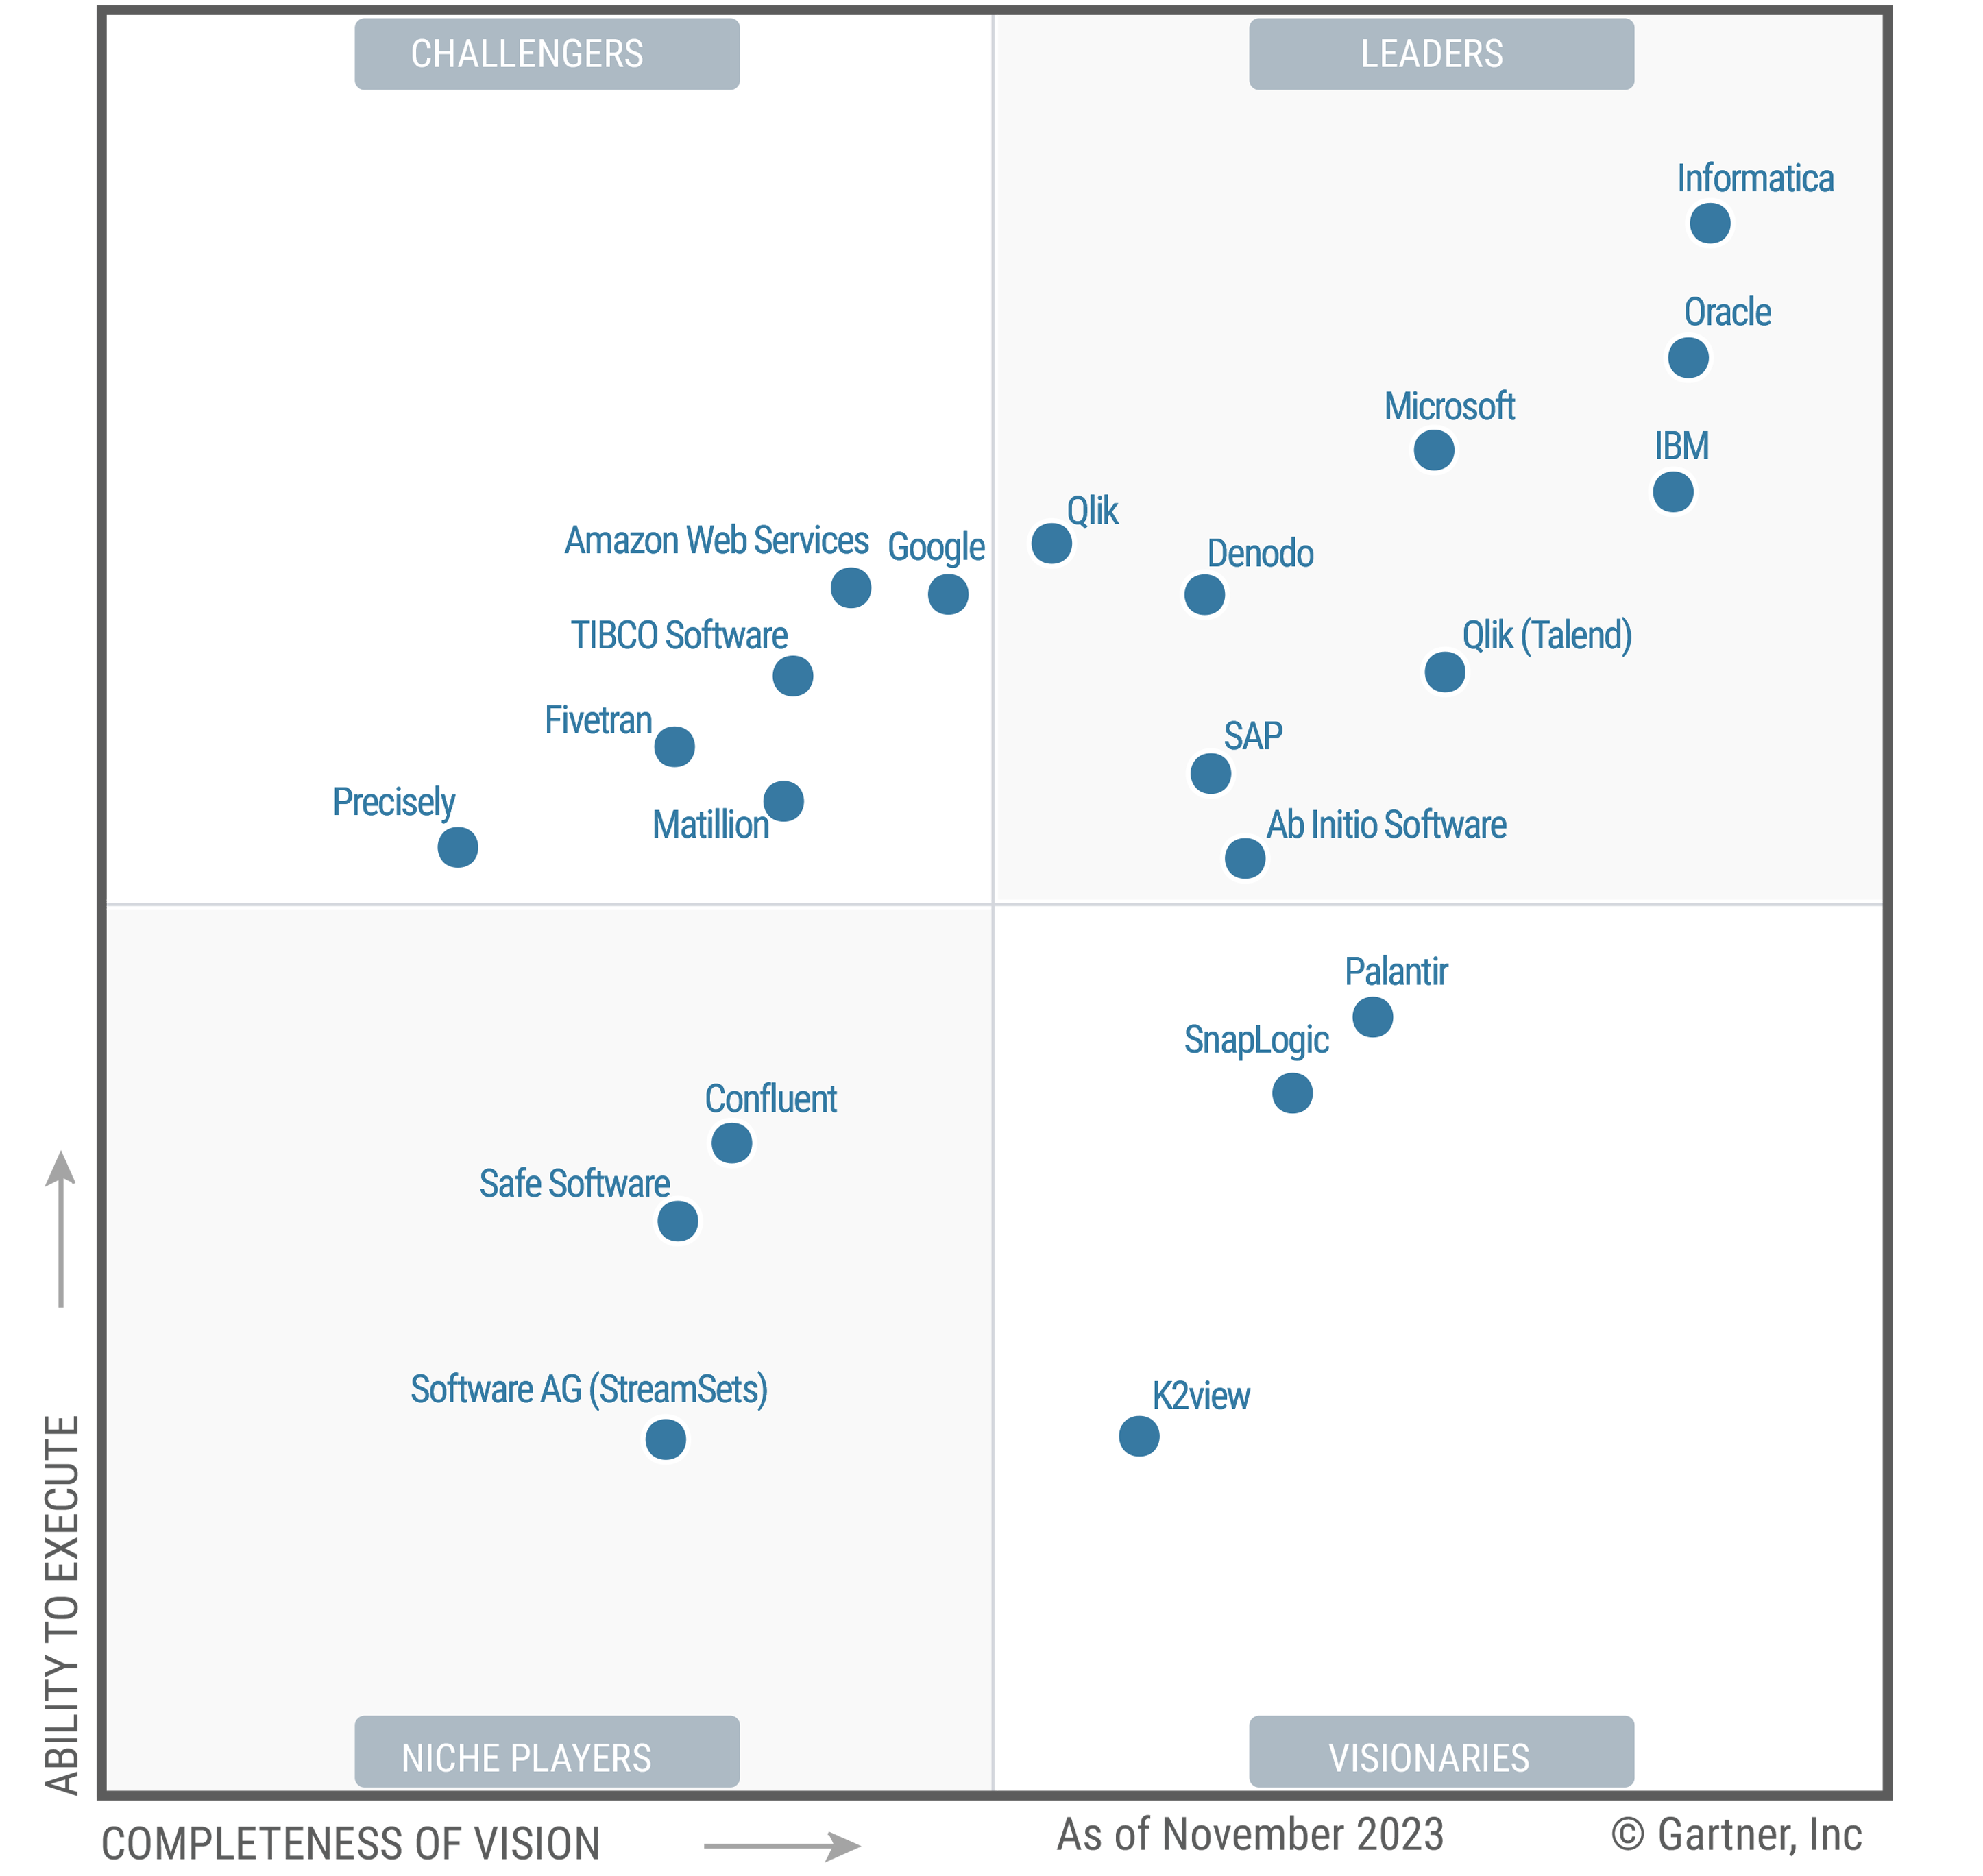
\includegraphics[width=0.65\linewidth]{img/gartner-data-integration.png}
    \caption{Gartner Data integration Magic Quadrant, zdroj: Gartner, 2023}
    \label{fig:datInteg}
\end{figure}

Tyto nástroje si podrobněji rozebereme a vzájemně porovnáme jejich schopnost splnit zmíněnou podmínku č. 1.

\subsection{MS-SQL Server Integration Services (SSIS)}

Microsoft SQL Server Integration Services (SSIS) je platforma pro vývoj podnikových řešení pro extrakci, transformaci a načítání dat (ETL). SSIS je součástí produktu Microsoft SQL Server, což je databázový a~analytický systém\footnote{Více informací na \url{https://www.microsoft.com/en-us/sql-server}}.

\subsubsection{Extrakce dat}
SSIS umožňuje extrakci dat z různých zdrojů, jako jsou relační databáze, XML soubory, webové služby a~další \cite{SQLServerDataSources:online}.
Tento proces je zásadní pro shromažďování dat z~různých zdrojů do jednoho úložiště ve formě, která je vhodná pro další zpracování.

\subsubsection{Transformace dat} Po extrakci dat SSIS poskytuje nástroje pro čištění, normalizaci, agregaci a další transformace dat. To zahrnuje operace jako spojení dat, rozdělení dat, nahrazení hodnot a~mapování dat \cite{SSISDataMapping:online}, pro což SSIS nabízí vizualní editor, jak ilustruje obrázek \ref{fig:SSISColumnMapping}.

\begin{figure}
    \centering
    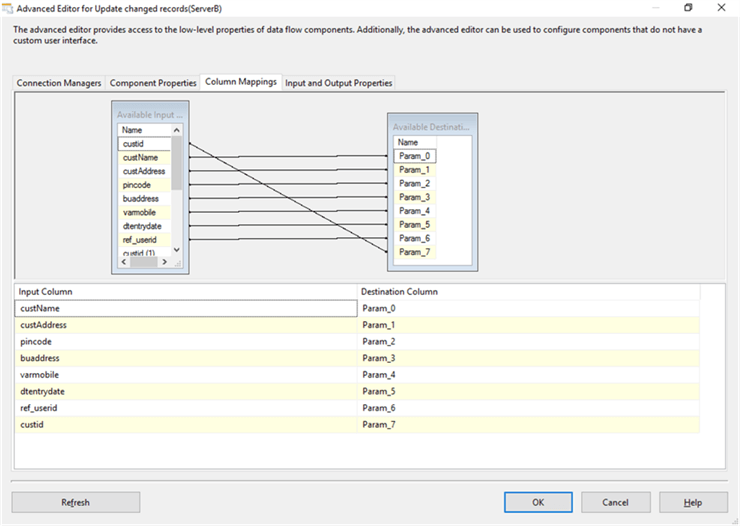
\includegraphics[width=0.75\linewidth]{img/SSIS column mapping.png}
    \caption{Mapování sloupců v SSIS, zdroj: Patel Bhavesh, 2017, dostupné z \url{https://www.mssqltips.com/tipimages2/5082_synchronization-jtk.012.png}}
    \label{fig:SSISColumnMapping}
\end{figure}

\subsubsection{Automatizace a orchestrace} SSIS také poskytuje nástroje pro automatizaci a orchestraci\footnote{Více na \url{https://cs.wikipedia.org/wiki/Orchestrace_(informatika)}} celého procesu ETL. To zahrnuje plánování úloh, sledování výkonu a řízení chyb.

\subsubsection{Integrace s dalšími nástroji Microsoft} Jako součást ekosystému Microsoft SQL Server SSIS se dobře integruje s dalšími nástroji Microsoft, jako jsou SQL Server Analysis Services (SSAS) a~SQL Server Reporting Services (SSRS).

\subsubsection{Vytvoření databázových pohledů}
Pomocí grafického editoru SSIS Designer můžeme přehledně vytvářet integrační balíčky~\cite{SSISDesigner:online}, prostředí SSIS Designer ilustruje obrázek \ref{fig:SSISDesigner}.
Tyto balíčky lze dle návodu z~edukačních stránek Microsoftu publikovat jako databázové pohledy~\cite{SSISViews:online}. 

Tímto postupem lze splnit 1.~funkční požadavek definovaný v~úvodním textu této kapitoly.

\begin{figure}
    \centering
    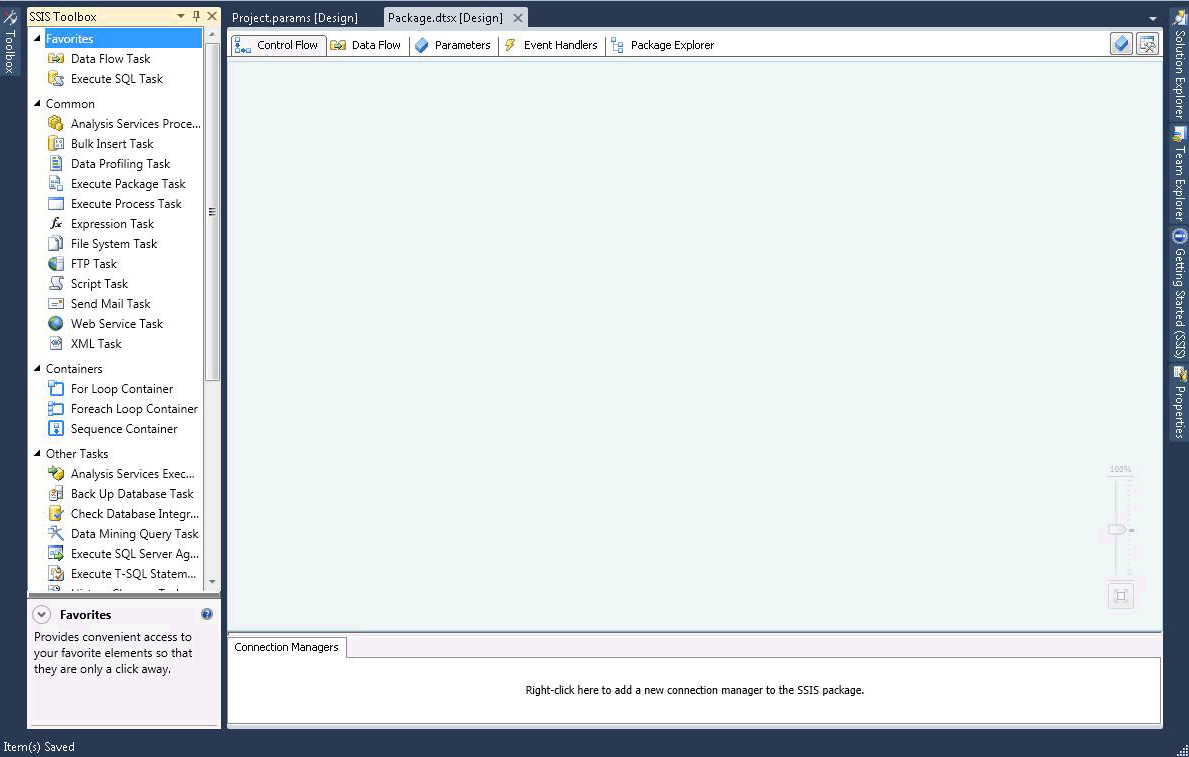
\includegraphics[width=0.75\linewidth]{img/SSIS Designer.png}
    \caption{Prostředí nástroje SSIS Designer, zdroj: Microsoft, 2023, dostupné z: \url{https://learn.microsoft.com/en-us/sql/integration-services/media/denali-designerandtoolbox.gif}}
    \label{fig:SSISDesigner}
\end{figure}

\subsubsection{Shrnutí}
MS-SQL Server Integration Services je silný nástroj pro podnikové ETL řešení a~mimo jiné i~pro náš případ.
Jeho schopnosti extrakce, transformace a~načítání dat, spolu s~funkcemi pro automatizaci a~integraci s~dalšími nástroji Microsoft, z~něj činí jeden z~klíčových nástrojů pro správu a~analýzu dat.


\subsection{Talend Open Studio}

Talend Open Studio je open-source platforma pro ETL. Tento nástroj je široce používán a~patří mezi nejlepší open-source nástroje na integraci dat \cite{TalendReview:online}.

\subsubsection{Extrakce dat}
Open Studio podporuje širokou škálu zdrojů dat, jako jsou relační databáze, jiné aplikace pracující s daty, webové služby a další \cite{TalendSupportedSources:online}. Prostředí nástroje ilustruje obrázek \ref{fig:TalendJobDesigner}

\begin{figure}
    \centering
    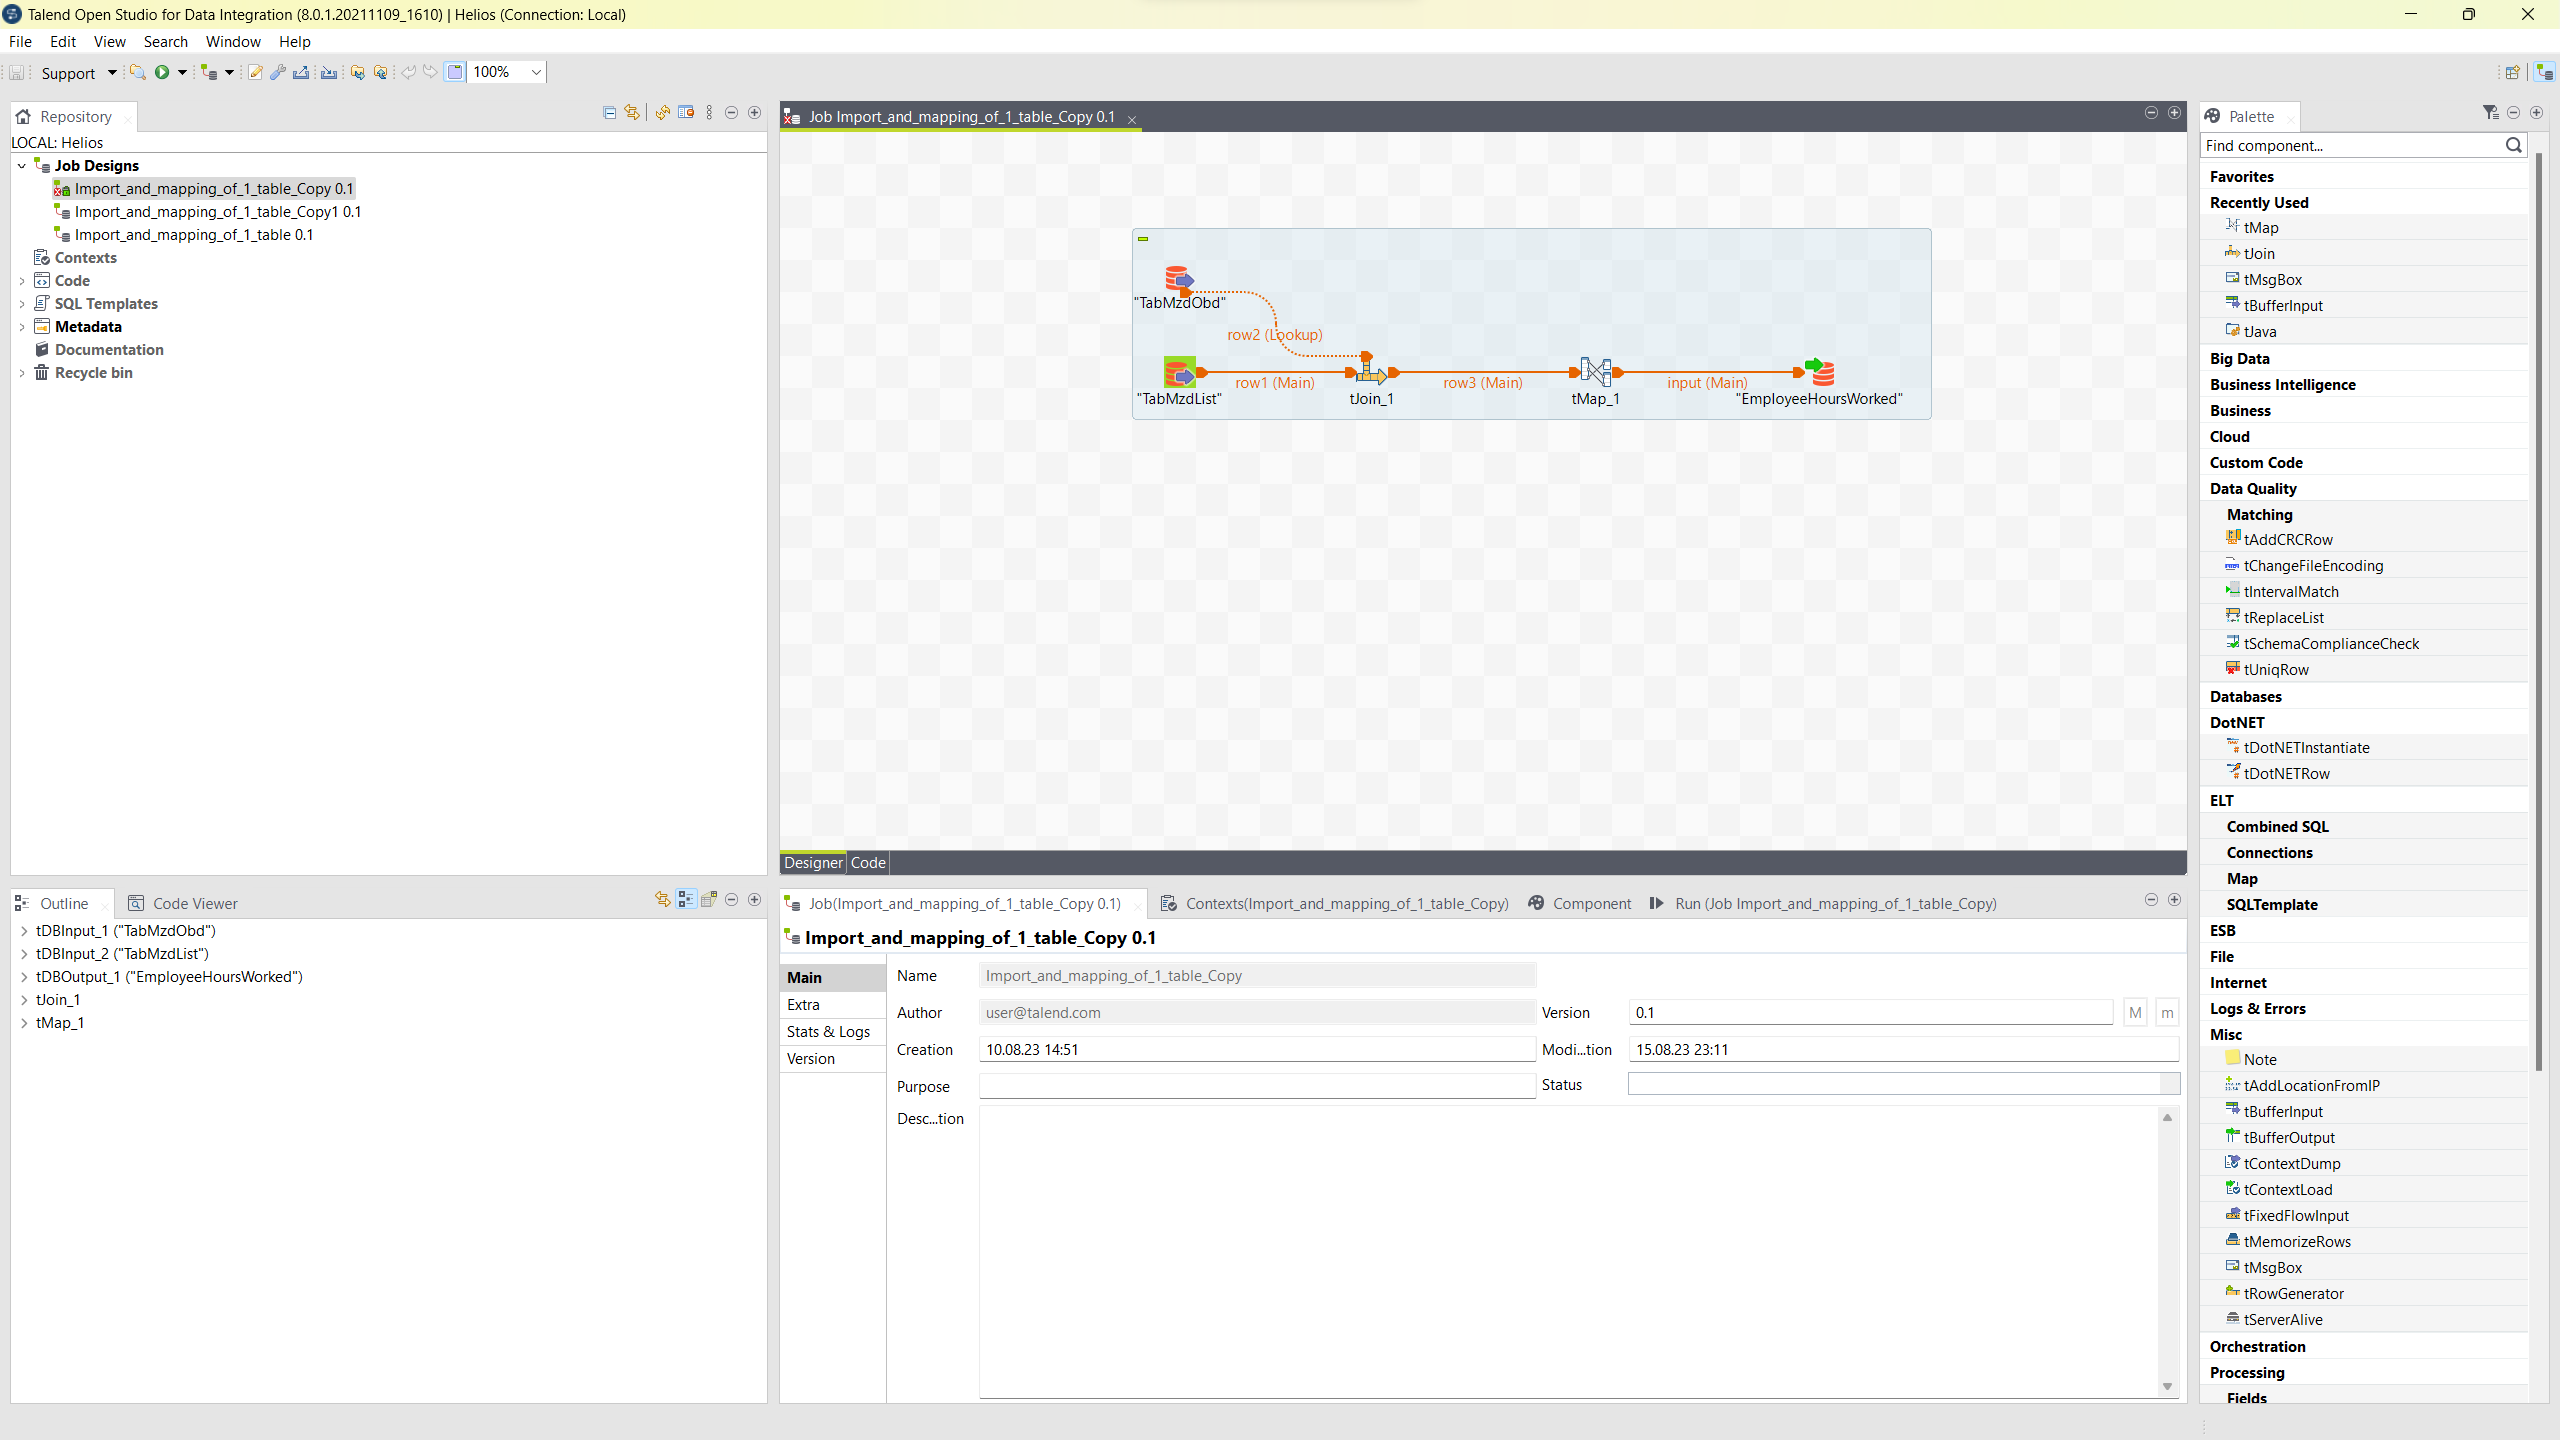
\includegraphics[width=0.75\linewidth]{img/Talend prostředí.png}
    \caption{Prostředí nástroje Talend Open Studio - Job Designer, zdroj: pořízeno autorem práce}
    \label{fig:TalendJobDesigner}
\end{figure}

\subsubsection{Transformace dat}
Podobně jako SSIS i Open Studio celou řadu nástroje pro čištění, normalizaci, agregaci a další transformace dat.
V rámci pro nás důležitého mapování dat Open Studio nabízí grafický editor, jak ukazuje obrázek \ref{fig:TalendColumnMapping}.

\begin{figure}
    \centering
    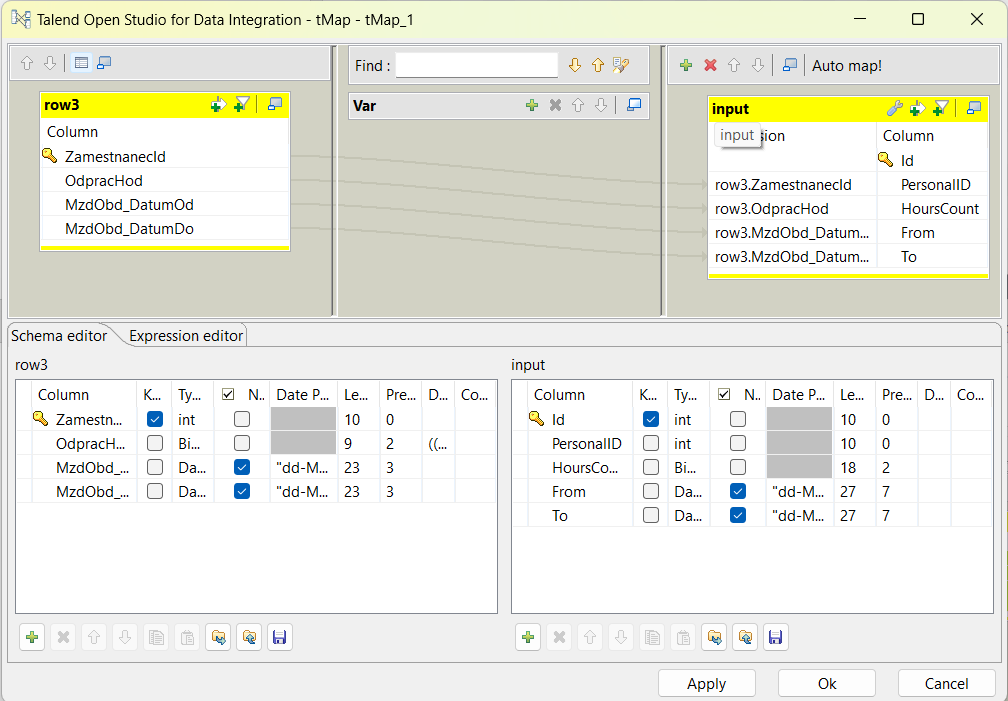
\includegraphics[width=0.6\linewidth]{img/Talend Column mapping.png}
    \caption{Mapování sloupců v Talend Open Studiu, zdroj: pořízeno autorem práce}
    \label{fig:TalendColumnMapping}
\end{figure}

\subsubsection{Automatizace a orchestrace}
Talend Open Studio také podporuje automatizaci celého ETL procesu.
Jednotlivé úlohy lze rozdělit do tzv. \textit{jobs} (jednotek práce), jejich exekuce může být periodicky plánována či podmíněna nějakou událostí \cite{TalendBuildingJobs:online}.

\subsubsection{Integrace s cloudem}
Talend Open Studio je kompatibilní s cloudovými službami, jako je AWS\footnote{Více informací na \url{https://aws.amazon.com/}} nebo Azure\footnote{Více informací na \url{https://azure.microsoft.com/}}, což umožňuje snadnou škálovatelnost a~zjednodušuje údržbu takového řešení \cite{TalendCloudInte:online}.

\subsubsection{Vytvoření databázových pohledů}
V~Open Studiu za pomocí ELT komponent dokážeme také vytvořit databázový pohledy \cite{TalendETL:online}.
Avšak ne tak jednoduše jako v~případě SSIS.

\subsubsection{Shrnutí}
Talend Open Studio je silný nástroj pro podnikové řešení ETL. Jeho schopnosti extrakce, transformace a načítání dat, spolu s~funkcemi pro automatizaci a~integraci s cloudovými službami, z~něj činí jeden z klíčových open-source nástrojů pro správu a~analýzu dat.

\subsection{Srovnání}\label{subsec:DataIntegComparison}
Podpora komunitních komponent dělá z Open Studia velmi versatilní nástroj, krom toho působí uživatelsky přívětivějším a přehlednějším dojmem než-li SSIS.
V neposlední řadě je nemalým benefitem možnost využít open-source verzi tohoto nástroje.

Na druhou stranu SSIS je velmi robustní nástroj, který nabízí obdobnou funkcionalitu jako Open Studio a navíc velmi snadnou integrovatelnost s rodinou nástrojů Microsoftu, což z něj dělá perfektní volbu při využití s~Power BI (viz podsekce \ref{subsec:PowerBI}).

Z~výše uvedeného nelze definitivně říct, že je jeden nástroj obecně lepší než druhý, tudíž volba závisí hlavně na kontextu užití.

\section{BI nástroje}\label{sec:BITools}
Sektor BI nástrojů je velmi rozsáhlý a probíhá v něm neustálý vývoj. Inspirujme se tedy výběrem nástrojů z~oblasti BI od firmy Gartner Inc \cite{FIG:BiTools}, který ilustruje obrázek \ref{fig:BITools}.

\begin{figure}[hp]
    \centering
    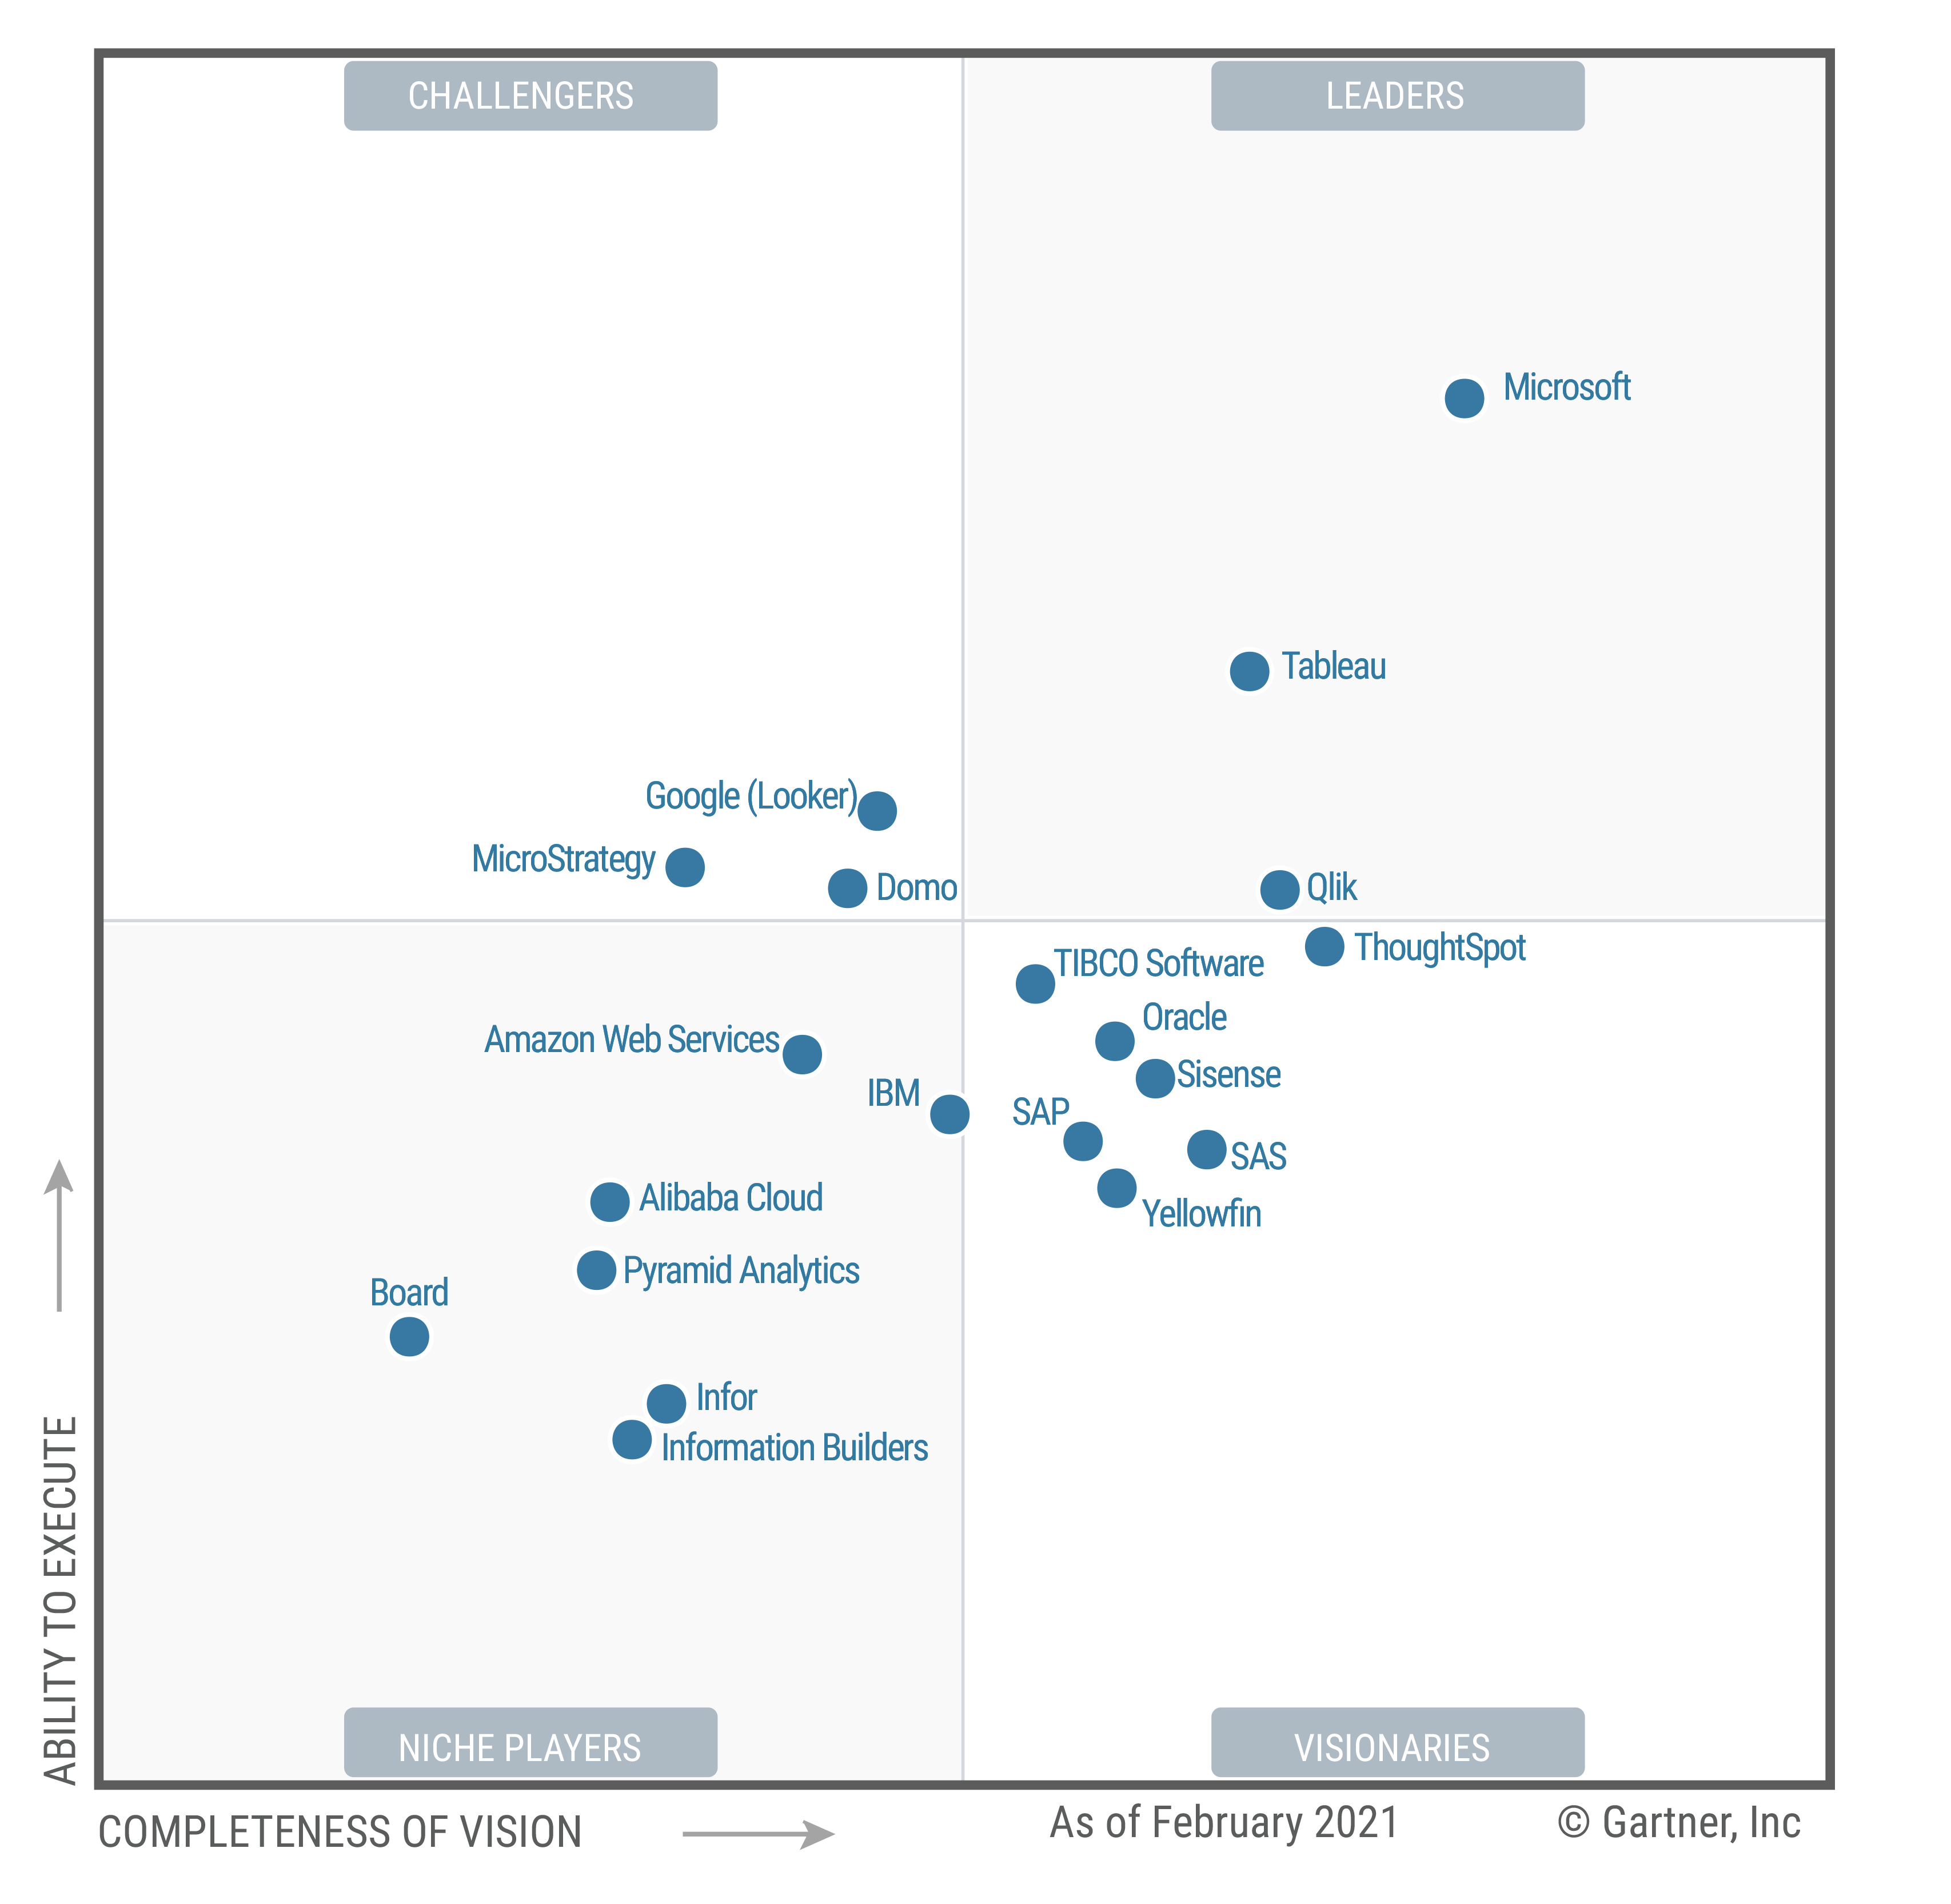
\includegraphics[width=0.6\linewidth]{img/gartner-BI-tools.png}
    \caption{Gartner BI Magic Quadrant, zdroj: Gartner, 2021}
    \label{fig:BITools}
\end{figure}

Výběr označuje nástroje \textit{Microsoft Power BI} a \textit{Tableau Desktop} jako lídry daného sektoru. Krom těchto dvou je pro kontext naší práce také zajímavý nástroj \textit{Metabase}, který budeme integrovat do našeho systému.

Zmíněné nástroje si podrobněji rozebereme v následujících podsekcích a uvedeme, jak splňují požadavky na funkcionalitu z \hyperref[chap:analysis]{úvodu kapitoly}.

\subsection{Microsoft Power BI}\label{subsec:PowerBI}
Microsoft Power BI je nástroj pro business intelligence, který nabízí interaktivní vizualizace dat a schopnosti business analytics\footnote{Řešení manažerských a obchodních problému za pomoci analýzi dat.} s rozhraním dostatečně jednoduchým pro koncové uživatele k vytváření svých vlastních zpráv a dashboardů.

Power BI je nejpoužívánějším nástrojem pro business intelligence na trhu~\cite{BIMarketShares:online} a~má hodnocení 4,4~hvězdiček z~5 z~více než 3~000 recenzí na platformě firmy Gartner Inc.~\cite{PowerBIReviews:online}.

\subsubsection{Podporované zdroje dat}
Power BI umožňuje uživatelům připojit se k různým datovým zdrojům, včetně Excelu, SQL Serveru, SharePointu\footnote{Více informací na \url{https://www.microsoft.com/cs-cz/microsoft-365/sharepoint/collaboration}.} a mnoha dalším \cite{PowerBIDataSources:online}.

\subsubsection{Výhody}\label{subsubsec:PowerBITemplates}
Power BI dokáže zpracovat velké datové sady~\cite{PowerBIBigData:online}. Také nabízí pokročilé analytické funkce, jako jsou Quick Insights, AI Insights a Analyze feature, které umožňují uživatelům snadno najít zajímavé informace a trendy v datech~\cite{PowerBIInsights:online}. Dále umožňuje vytvářet vizualizace pomocí předem vytvořených šablon nebo vlastních návrhů. Uživatelé mohou také vytvářet interaktivní dashboardy, které nabízejí rychlý přehled o klíčových ukazatelích výkonnosti~\cite{PowerBIBigData:online}.

Interaktivní dashboardy ilustruje obrázek \ref{fig:PowerBIUI}. 
\nocite{WhatisPowerBI:online}
\begin{figure}
    \centering
    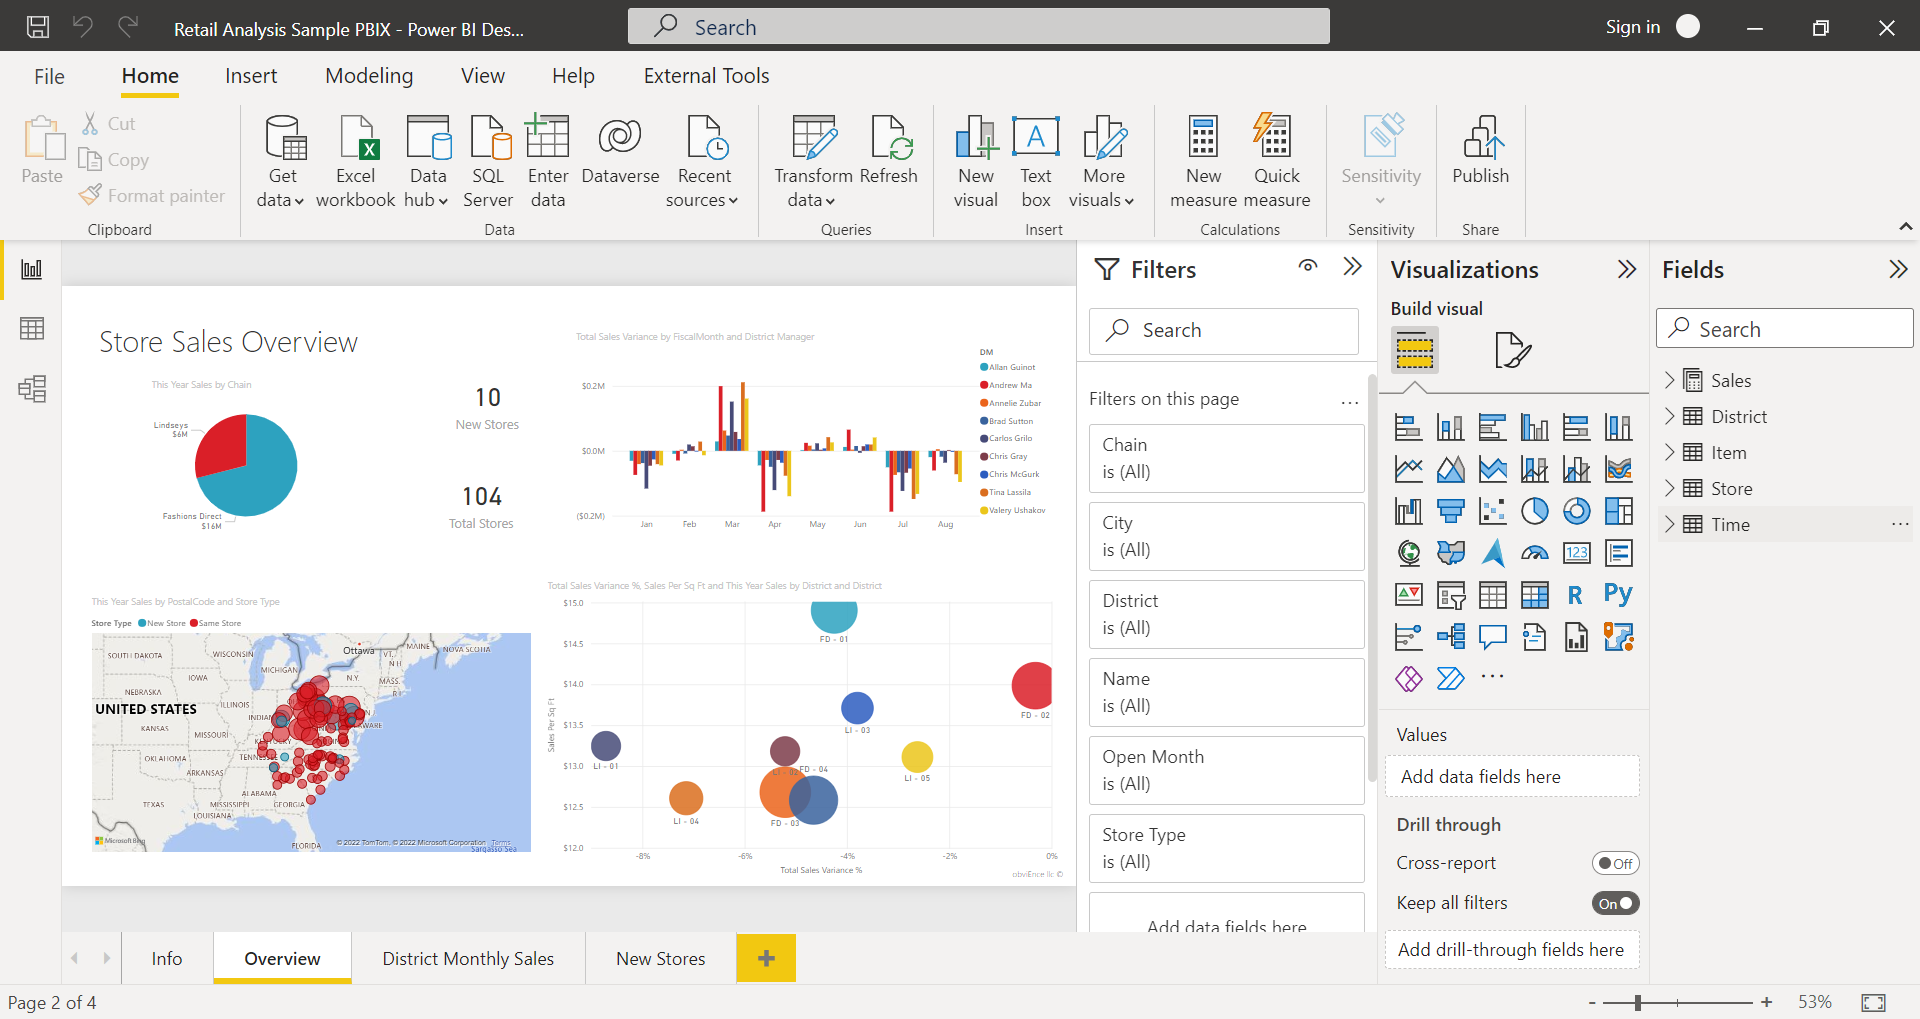
\includegraphics[width=0.75\linewidth]{img/PowerBIUI.png}
    \caption{Prostředí Power BI — vytváření nástěnky, zdroj: Microsoft, 2023, dostupné z: \url{https://learn.microsoft.com/en-us/power-bi/fundamentals/media/desktop-what-is-desktop/what-is-desktop-01.png} }
    \label{fig:PowerBIUI}
\end{figure}

\subsubsection{Určení}
Power BI je zejména vhodný pro střední až větší firmy, v nichž je potřeba rychle vytvářet vizualizace a nástěnky bez nutnosti rozsáhlého školení. Pro zkušenější uživatele nabízí řadu pokročilejších funkcí\cite{PowerBIBigCompanies:online}.

\subsubsection{Shrnutí}
Microsoft Power BI je velmi oblíbený nástroj pro business intelligence, který nabízí jak základní funkcionalitu většiny BI nástrojů, tak pokročilé analytické funkce, jako jsou Quick Insights, AI Insights a Analyze feature.

Co se týče našich požadavků na funkcionalitu, Power BI rozhodně oba dva splňuje, přičemž přenositelnost je zajištěna možností vytvářet a využívat zmíněné \hyperref[subsubsec:PowerBITemplates]{šablonové řešení}.

\subsection{Tableau}
-
% Tableau Desktop je výkonný nástroj pro vizualizaci dat, který umožňuje připojení, analýzu a vizualizaci jakýchkoli dat.

\subsubsection{Podporované zdroje dat}
-
% Připojení k datům: Tableau Desktop umožňuje připojení k datům jak na místě (on-premise), tak v cloudu.

\subsubsection{Výhody}
-
% Analýza dat: Uživatelé mohou provádět pokročilé analýzy, vytvářet vypočítaná pole, hledat shluky v datech, počítat procenta a používat různé nástroje k prozkoumání a kontrole dat2. Tableau Desktop také nabízí funkci výrazů úrovně detailu (LOD), které umožňují výpočty na úrovni zdroje dat a vizualizace.

% Vizualizace dat: S intuitivním rozhraním přetahováním a pomocí dynamických náhledů mohou uživatelé snadno vytvářet a iterovat vizualizace.

% Automatizované doplňkové informace: Tableau Desktop pomáhá lidem na všech úrovních dovedností lépe rozhodovat s daty. Nabízí zkušenosti zlepšené umělou inteligencí a strojovým učením, které vedou obchodní uživatele k odpovědím, které potřebují.

\subsubsection{Určení}
-
% Sdílení a spolupráce: Uživatelé mohou bezpečně sdílet analýzy a náhledy připojením k Tableau Serveru nebo Tableau Cloud.

\subsubsection{Shrnutí}
-
% Tableau Desktop je tedy komplexní nástroj, který nabízí širokou škálu funkcí pro práci s daty, od připojení k datům až po sdílení výsledků analýzy. Je to jakýsi laboratoř, ve které můžete objevovat význam, který se skrývá ve vašich datech

\subsection{Metabase}
- 
% Metabase je platforma pro analýzu dat, která umožňuje vyhledávání dat na vysoké úrovni po celém pracovním prostoru nebo detailnější dotazy, které lze vytvořit pomocí nízko-kódového SQL dotazovacího nástroje. 

\subsubsection{Podporované zdroje dat} 
- 
% Metabase podporuje mnoho různých databází a datových skladů, což umožňuje prozkoumávat a učit se z dat, bez ohledu na to, kde jsou uložena1. Mezi podporované zdroje dat patří: ...

\subsubsection{Výhody} 
- 
% Metabase je oblíbený pro své uživatelsky přívětivé rozhraní, snadnou navigaci a cenovou dostupnost jako nástroj s otevřeným zdrojovým kódem10. Další výhody zahrnují: 

% Snadné použití: Metabase je velmi snadno použitelný a ideální pro marketingové a obchodní profesionály všech úrovní. 

% Flexibilita: Metabase je známý svou flexibilitou pro více podniků v různých odvětvích nebo oblastech, stejně jako pro celkovou velikost organizace

% Podpora prostředí: Metabase je snadno nasaditelný a použitelný i pro netechnické uživatele díky podpoře prostředí. 

% Vizualizace dat: Metabase nabízí širokou škálu nástrojů pro vizualizaci dat, které umožňují vytváření komplexních zpráv a řídicích panelů. 

\subsubsection{Určení} 
- 
% Metabase je zaměřen na týmy pro analýzu dat v organizaci5. Je ideální pro malé a střední podniky, startupy nebo týmy s omezenými znalostmi BI. 

\subsubsection{Shrnutí}
- 
% Metabase je komplexní nástroj, který nabízí širokou škálu funkcí pro práci s daty, od připojení k datům až po sdílení výsledků analýzy. Jeho snadné použití, flexibilita a široká podpora datových zdrojů ho činí silným nástrojem pro jakoukoli organizaci, která se snaží získat cenné informace z jejích dat. 

% \subsubsection{TODO}
% SaaS deployment manažer
% Vzpomenout ten v Go,
% Mnoho nepotřebných features

\section{Závěr}\label{sec:AnalysEnd}

V předchozích sekcích jsme si představili několik nástrojů, jejichž kombinací lze splnit požadavky na funkcionalitu definované v~\hyperref[chap:analysis]{úvodním textu} této kapitoly. 
Ovšem kombinace těchto nástrojů by vytvářela poměrně nesourodý celek, který by bylo složité automatizovat a~integrovat do jednoho systému. 

Další problém představují nástroje na integraci dat.
Jsou totiž spíše určeny pro použití experty na integraci či analýzu dat, proto je u~nich kladen důraz na obecnost a~širokou škálu využití, a~tak pro náš systém mnohonásobně převyšují požadovanou funkcionalitu.
Tato nepotřebná funkcionalita přidává na komplexitě těchto nástrojů, což vytváří barieru pro použití ve spolupráci se zákazníkem - laikem.

V dalších kapitolách se tedy budeme soustředit na navržení a~implementaci vlastního řešení, které minimalizuje nabízenou funkcionalitu na nezbytně nutnou úroveň, jež splňuje funkční požadavky, za účelem zachování jednoduchosti použití.
Krom toho se budeme snažit vyhovět dalším požadavkům \textit{Firmy} na vlastní řešení.

Kdybychom přeci jen měli vybrat nejlepší hledanou kombinaci z představených nástrojů, byly by jí nástroje \textit{SSIS} a \textit{Power BI} od Microsoftu, které díky jednotnému původu nabízí nejsnadnější integrovatelnost.

%%% Fiktivní kapitola s ukázkami citací

\chapter{Definice požadavků}\label{chap:requirements}

Abychom navrhli a~implementovali v~praxi použitelný systém, musíme nejprve podrobněji rozebrat, jaké požadavky jsou na systém kladeny. 

\section{Funkční požadavky}

Jednotlivé funkční požadavky si představíme ve formě uživatelských příběhů (anglicky \textit{user stories}).
Jak uvádí Fred Health, jedná se o~formu zaznamenávání funkčních požadavků na systém ve strukturované podobě krátkých příběhů většinou vypadajících následovně: 

„Jako \textit{typ uživatele} chci, nebo potřebuji \textit{nějakou funcionalitu}, aby \textit{nějaký benefit}.“\cite{userStories}  

Tato forma zápisu nám pomůže konzistentně strukturovat informace o~tom, jakou funkcionalitu potřebuje jaký typ uživatele a~proč ji daný typ uživatele potřebuje, což zužitkujeme při tvorbě designu systému (viz kapitola \ref{chap:design}).

Definujeme si 2 typy uživatelů systému:

\begin{itemize}
    \item Zákazník — je uživatel využívající systém pro mapování a~vizualizaci dat.
    \item Správce systému — je zaměstnanec provozovatele systému, který má na starost správu zákazníků a~poskytování asistence s~jejich problémy.
\end{itemize}

Dále si upřesníme některé pojmy, jež budeme v~příbězích užívat:

\begin{itemize}
    \item Nový zákazník — je zákazník, s~nímž byla nově domluvena spolupráce a~ještě pro něj není vytvořený uživatelský účet.
    \item Stávající zákazník — je zákazník, pro něhož je vytvořený účet a~může používat všechny části systému, tzn. již pro něj je dostupná instance nástroje \textit{Metabase}. 
    \item Bývalý zákazník — je zákazník, s~nímž byla spolupráce rozvázána.
    \item Mapování dat — je dle Wikipedie proces vytváření mapování mezi elementy dvou datových modelů, např. za účelem pozdější tranformace dat mezi danými datovými modely\cite{dataMapping:online}.
    My se omezíme na mapování mezi relačními modely.
    
    \item Generický datový model — je datový model, který je dostatečně zobecněný, abychom na něj mohli převést, v našem případě, data od různých zákazníků.
    \item Mapovací nástroj — je jeden z~modulů našeho systému, který umožňuje zákazníkům mapovat data na generický datový model systému.
    \item Mapovací projekt — označení pro mapování dat jednoho zákazníka na generický datový model systému.
    \item Klastr — pojemem klastr (anlgicky \textit{cluster}) je myšlen Kubernetes klastr\footnote{Více informací v podsekci \ref{subsec:k8s}.}.
    \item Dashboard - je dle Wikipedie typ grafického UI, který umožňuje jednoduše na jednom místě sledovat hlavní ukazatele výkonnosti\footnotemark{} dané organizace ve strukturované podobě \cite{Dashboards:online}.
    V našem případě se bude jednat o~dashboardy z nástroje \textit{Metabase}.
\end{itemize}
\footnotetext{Více na \url{https://en.wikipedia.org/wiki/Performance_indicator}.}

Uživatelské příběhy rozdělíme do dvou následujících podsekcí podle typu uživatele.



\subsection{Příběhy správce systému}

\begin{enumerate}
    \item Jako správce systému potřebuji přidávat \textit{nové zákazníky}, aby mohli začít používat systém.
    \item Jako správce systému potřebuji mazat \textit{bývalé zákazníky}, aby jen \textit{stávající zákazníci} měli přístup do systému.
    \item Jako správce systému potřebuji nahlížet do \textit{mapovacích projektů} zákazníků, abych mohl poskytnout asistenci s mapováním nebo mohl provést kontrolu \textit{mapování}.
    \item Jako správce systému potřebuji zajistit spuštění nové instance nástroje \textit{Metabase} v \textit{klastru}, aby jej zákazník  mohl začít používat.
    \item Jako správce systému potřebuji, aby systém v případě spuštění nové instance nástroje \textit{Metabase} automaticky provedl zpracování mapování a zpřístupnil vizualizaci dat daného zákazníka pomocí nové instance.
    \item Jako správce systému potřebuji, aby systém vyžadoval přihlášení po všech uživatelích, aby uživatelská data nebyla zpřístupněna neoprávněným osobám.
    \item Jako správce systému v případě, kdy zákazník odejde od \textit{Firmy}, potřebuji, aby systém ukončil instanci nástroje \textit{Metabase} příslušící danému uživateli, aby jej již nemohl používat.
    
\end{enumerate}

Příběhy správce jsou shrnuty formou use case diagramu\footnote{
Diagram případů užití (anglicky \textit{use case diagram}) je v softwarovém inženýrství jeden z~UML diagramů chování \cite{useCaseDiagWiki:online}.
}
na obrázku \ref{fig:admin-use-cases}.
\begin{figure}
    \centering
    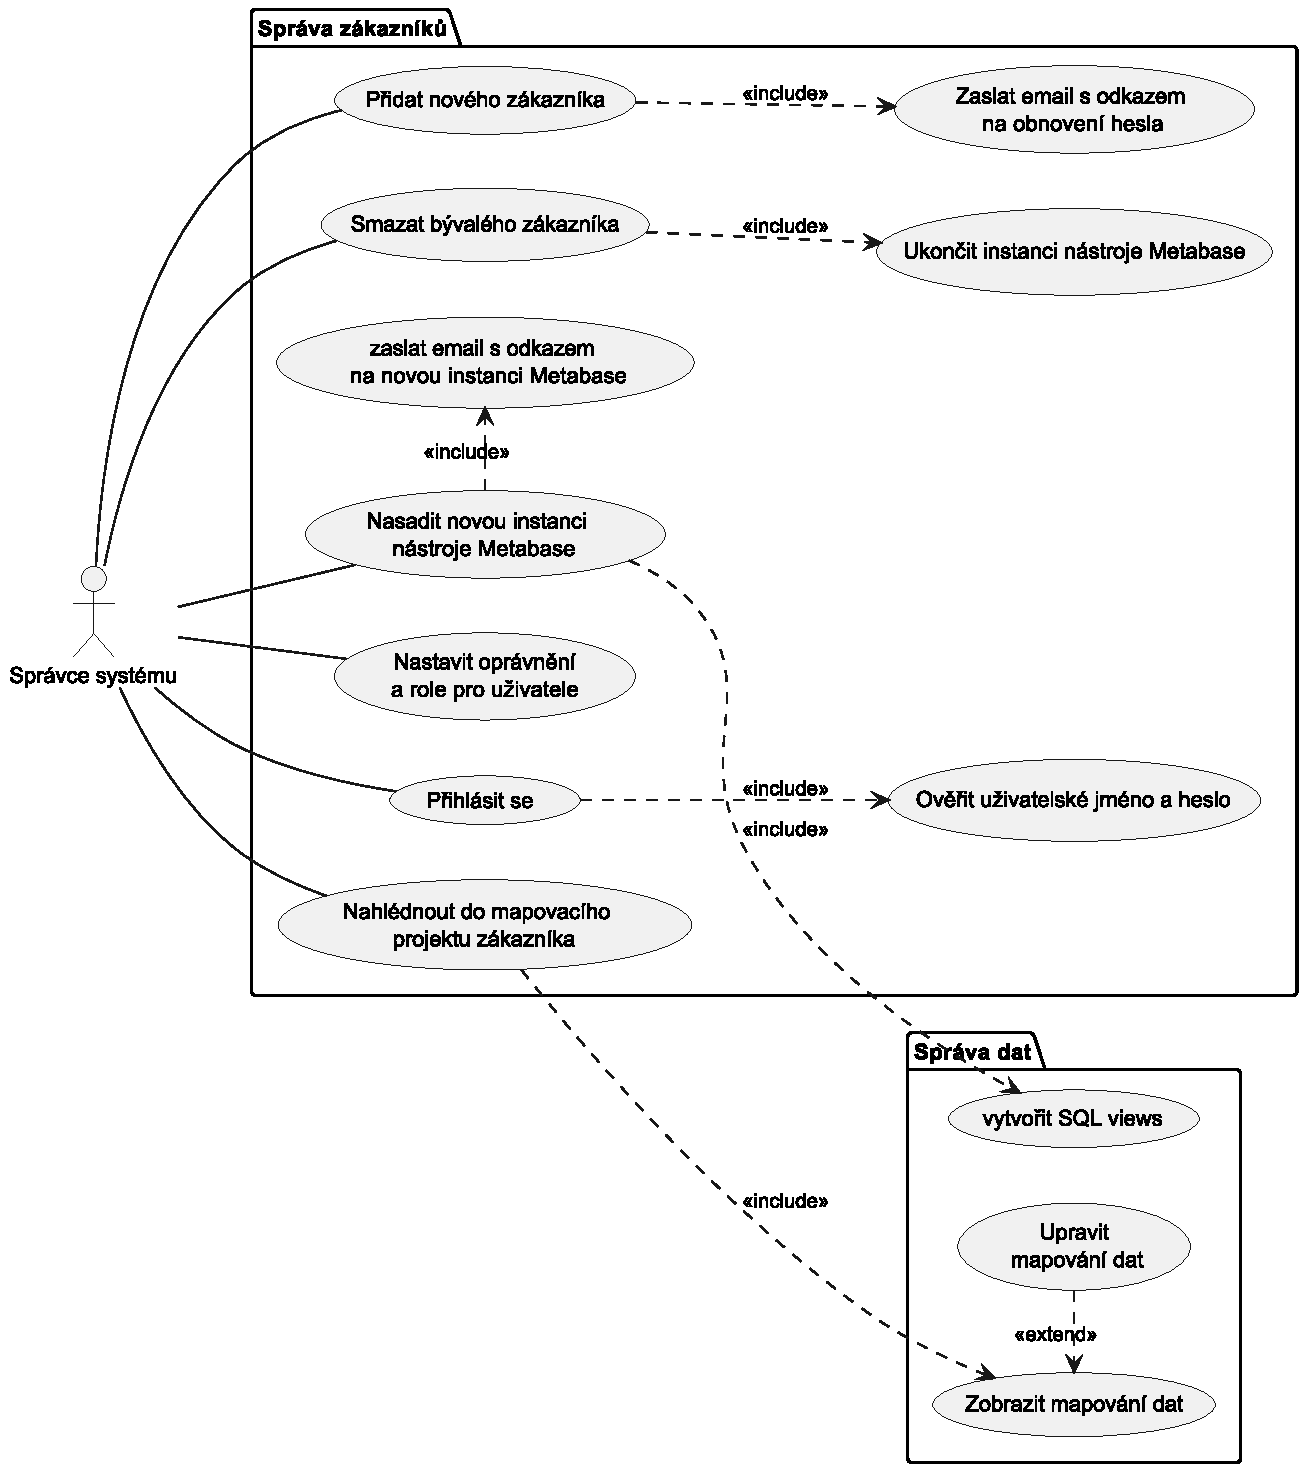
\includegraphics[width=\linewidth]{img/Use Case Diagram - Správce systému (1).pdf}
    \caption{Diagram případů užití systému správcem}
    \label{fig:admin-use-cases}
\end{figure}

\subsection{Zákaznické příběhy}

\begin{enumerate}
    \item Jako zákazník potřebuji připojit svoji Microsoft SQL Server\footnote{Více na \url{https://www.microsoft.com/cs-cz/sql-server}} databázi ERP systému k systému, abych mohl začít mapovat svoje data na \textit{generický datový model}.
    \item Jako zákazník potřebuji používat uživatelsky přívětivý \textit{nástroj pro mapování dat}, abych mohl snadno a~rychle převést svoje data na generický datový model.
    \item Jako zákazník potřebuji mít možnost zadat přístupové ke své databázi, aby systém mohl připravit mapování dat.
    \item Jako zákazník potřebuji mít možnost upravovat nebo změnit mapování dat, abych mohl reagovat na změny v~mých datech nebo požadavcích.
    \item Jako zákazník potřebuji mít přístup k nástroji \textit{Metabase}, abych mohl vizualizovat a~analyzovat svoje data pomocí různých reportů a dashboardů.
    \item Jako zákazník potřebuji mít možnost sdílet nebo exportovat svoje reporty a~dashboardy, abych mohl prezentovat nebo sdílet svoje výsledky s~ostatními.
    \item Jako zákazník potřebuji mít možnost poskytnout zpětnou vazbu nebo požádat o~podporu, abych mohl řešit případné problémy nebo potřeby v rámci systému.
\end{enumerate}

Výše uvedené požadavky zjednodušeně ilustruje use case diagram \ref{fig:customer-use-cases}.

\begin{figure}
    \centering
    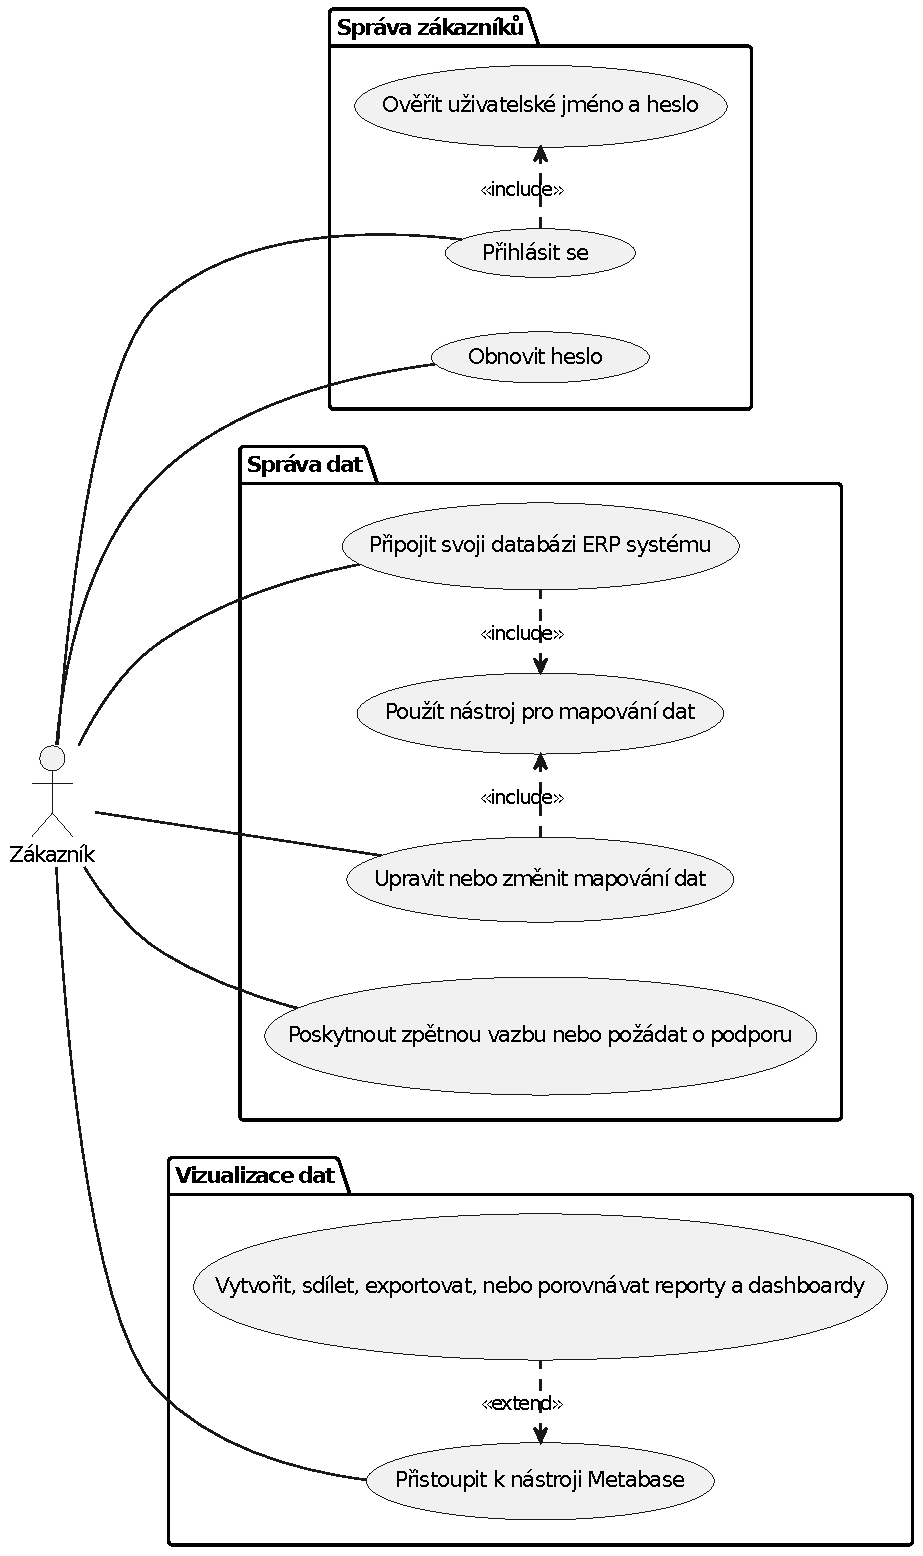
\includegraphics[width=0.75\linewidth]{img/Use Case diagram - Zákazník (2).pdf}
    \caption{Diagram případů užití systému zákazníkem}
    \label{fig:customer-use-cases}
\end{figure}


\section{Nefunkční požadavky}

Podle Sommervilla jsou nefunkční požadavky\footnote{Z anglického \textit{non-functional requirements}.} omezení kladená na systém jako celek spíše než požadavky na jednotlivé funkce systému.
Sommerville dále uvádí, že tyto požadavky jsou mnohdy zásadnější než mnohé funkční požadavky \cite{Sommerville}(strana 85-88), tudíž i~my si patřičně rozebereme, jaké nefunkční požadavky musí námi vyvíjený systém splňovat.

Typů nefunkčních požadavků existuje celá řada~\cite{NonFunct69:online}, jak ilustruje obrázek \ref{fig:non-func-types}. My se tudíž v~následujících podsekcích zaměříme jen na několik hlavních.

\begin{figure}
    \centering
    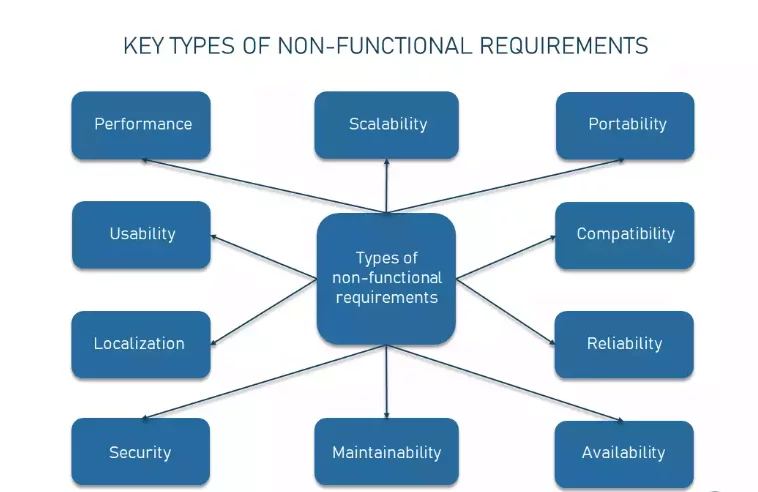
\includegraphics[width=0.75\linewidth]{non-functional-req-types.png}
    \caption{Základní typy nefunkčních požadavků, zdroj: Testomat.io, 2023, dostupné z~\url{https://testomat.io/wp-content/uploads/2023/03/Key_Software_Req.png}}
    \label{fig:non-func-types}
\end{figure}

\subsection{Výkonnost}
Jelikož se neočekává, že systém budou využívat stovky či tisíce uživatelů současně, požadavky na výkon jsou zaměřeny spíše na náročnější akce, které by měl systém vykonávat.

\begin{itemize}
    \item Nasazení nové instance nástroje Metabase nesmí trvat déle než 30 sekund.
    \item Vytvoření nového projektu zákazníka nesmí trvat déle než 30 sekund.
\end{itemize}

\subsection{Použitelnost}

Tento aspekt systému je zejména z pohledu zákazníka klíčový.
Konfigurace přístupových údajů k zákaznické databázi a mapování dat musí být co nejintuitivnější. 70~\% zákazníků musí tento proces zvládnout samostatně.

\subsection{Udržitelnost}

Systém musí být rozdělen do modulů a komponent, aby se snížila nutnost zasahovat do různých částí systému v případě změny v pouze určité části.

\subsection{Bezpečnost}

Jelikož pracujeme se zákaznickými daty, je naprosto zásadní, aby tato data zůstala chráněna.

\begin{itemize}
    \item Všichni uživatelé musí být autentizováni.
    \item Přístupové údaje daného zákazníka si může zobrazit a~modifikovat pouze daný zákazník.
    \item Zákazníci nesmí být schopni si navzájem nahlížet do mapování dat. 
\end{itemize}

\subsection{Interoperabilita}
\begin{itemize}
    \item Systém musí pro export mapování využívat formát JSON.
    \item Systém musí podporovat databázový systém \textit{Microsoft SQL Server} a být připraven na rozšíření podpory pro další databázové systémy.
\end{itemize}

\subsection{Škálovatelnost}

Systém musí být schopný provozovat 30 instancí nástroje \textit{Metabase} zároveň.

\subsection{Portabilita}

Systém musí podporovat jakoukoliv platformu, která umožňuje běh Docker kontejnerů\footnote{Více informací na \url{https://cs.wikipedia.org/wiki/Docker}.}.

\subsection{Testovatelnost}

Systém musí být obohacen o testovací data a testovací prostředí, které umožní běh celého systému pro integrační testování.
Kód systému musí využívat programovací techniky enkapsulace\footnote{Více informací na \url{https://en.wikipedia.org/wiki/Encapsulation_(computer_programming)}} pro usnadnění testování jednotlivých komponent.
%%% Fiktivní kapitola s ukázkami tabulek, obrázků a kódu

\chapter{Design systému}\label{chap:design}


%%% Fiktivní kapitola s instrukcemi k PDF/A

\chapter{Popis funkcionality}\label{chap:functionality}

%%% Fiktivní kapitola s ukázkami citací

\chapter{Implementace}\label{chap:implementation}

\section{Použité technologie}
\subsection{Kubernetes}\label{subsec:k8s}

\chapter{Testování}\label{chap:testing}

\chapter*{Závěr}\label{chap:sum}
\addcontentsline{toc}{chapter}{Závěr}


%%% Seznam použité literatury
%%% Seznam použité literatury (bibliografie)
%%%
%%% Pro vytváření bibliografie používáme bibTeX. Ten zpracovává
%%% citace v textu (např. makro \cite{...}) a vyhledává k nim literaturu
%%% v souboru literatura.bib.
%%%
%%% Příkaz \bibliographystyle určuje, jakým stylem budou citovány odkazy
%%% v textu. V závorce je název zvoleného souboru .bst. Styly plainnat
%%% a unsrt jsou standardní součástí latexových distribucí. Styl czplainnat
%%% je dodáván s touto šablonou a bibTeX ho hledá v aktuálním adresáři.

% \bibliographystyle{czplainnat}    %% Autor (rok) s českými spojkami
% \bibliographystyle{plainnat}    %% Autor (rok) s anglickými spojkami
\bibliographystyle{unsrt}       %% [číslo]

\renewcommand{\bibname}{Seznam použité literatury}

%%% Vytvoření seznamu literatury. Pozor, pokud jste necitovali ani jednu
%%% položku, seznam se automaticky vynechá.

\bibliography{literatura}

%%% Kdybyste chtěli bibliografii vytvářet ručně (bez bibTeXu), lze to udělat
%%% následovně. V takovém případě se řiďte normou ISO 690 a zvyklostmi v oboru.

% \begin{thebibliography}{99}
%
% \bibitem{lamport94}
%   {\sc Lamport,} Leslie.
%   \emph{\LaTeX: A Document Preparation System}.
%   2. vydání.
%   Massachusetts: Addison Wesley, 1994.
%   ISBN 0-201-52983-1.
%
% \end{thebibliography}


%%% Obrázky v bakalářské práci
%%% (pokud jich je malé množství, obvykle není třeba seznam uvádět)
\listoffigures

%%% Tabulky v bakalářské práci (opět nemusí být nutné uvádět)
%%% U matematických prací může být lepší přemístit seznam tabulek na začátek práce.
\listoftables

%%% Použité zkratky v bakalářské práci (opět nemusí být nutné uvádět)
%%% U matematických prací může být lepší přemístit seznam zkratek na začátek práce.
\chapwithtoc{Seznam použitých zkratek}

%%% Přílohy k bakalářské práci, existují-li. Každá příloha musí být alespoň jednou
%%% odkazována z vlastního textu práce. Přílohy se číslují.
%%%
%%% Do tištěné verze se spíše hodí přílohy, které lze číst a prohlížet (dodatečné
%%% tabulky a grafy, různé textové doplňky, ukázky výstupů z počítačových programů,
%%% apod.). Do elektronické verze se hodí přílohy, které budou spíše používány
%%% v elektronické podobě než čteny (zdrojové kódy programů, datové soubory,
%%% interaktivní grafy apod.). Elektronické přílohy se nahrávají do SISu a lze
%%% je také do práce vložit na CD/DVD. Povolené formáty souborů specifikuje
%%% opatření rektora č. 72/2017.
\appendix
\chapter{Přílohy}

\section{První příloha}

\openright
\end{document}
